\documentclass{crm-article}

\usepackage{graphicx}
\usepackage{amsmath} 
\usepackage{bm}
\usepackage{amsbsy} 
\usepackage{amssymb}
\usepackage{cite}
\usepackage{multirow}

\graphicspath{{./figs/}}


\begin{document}

%\englishpaper % раскомментировать в том случае, если текст статьи на английском языке

%\norussian % раскомментировать, если нет метаданных на русском

%\affiliationnoref % раскомментировать, если автор один или все авторы из одной организации

%\emailnoref % раскомментировать в том случае, если автор единственный

%\year=2018 % current year by default
\journalVol{10}
\journalNo{1} %выпуска
\setcounter{page}{1}

% раздел журнала
\journalSection{Математические основы и численные методы моделирования}
\journalSectionEn{Mathematical modeling and numerical simulation}


% дата получения
\journalReceived{01.12.2020.}
%\journalReviewed{01.06.2016.}
%принято к публикации
\journalAccepted{01.12.2020.}


\UDC{519.63}
\title{Численное моделирование нестационарных задач переноса нейтронов в $\mathrm{SP_3}$ приближении}
\titleeng{Numerical modeling of non-stationary problems of neutron transport in the $\mathrm{SP_3}$ approximation}
\thanks{Работа выполнена при поддержке гранта Российского Научного Фонда \#19-71-00008}%если имеется
\thankseng{This work was supported by the grant of the Russian Science Foundation \#19-71-00008}

%автор - в формате \author{\firstname{И.\,И.}~\surname{Иванов}}
\author{\firstname{Александр.\,В.}~\surname{Аввакумов}}
%автор - в формате \authorfull{Имя Отчество Фамилия}
\authorfull{Александр Владимирович Аввакумов}
% автор на англ. - в формате \authoreng{\firstname{I.\,I.}~\surname{Ivanov}}
\authoreng{\firstname{A.\,V.}~\surname{Avvakumov}}
%автор на англ. - в формате \authorfull{Firstname M. Surname}
\authorfulleng{Aleksandr V. Avvakumov}
%вписать свою электронную почту
\email{avvakumov2009@rambler.ru}
%организация - в формате \affiliation{Московский государственный университет,\protect\\ Россия, 141700, г. Москва, ул. Университетская, д. 9}
\affiliation{Национальный исследовательский центр <<Курчатовский институт>>,\protect\\ Россия, 123182, г. Москва, пл. Академика Курчатова, д. 1}
%организация - в формате \affiliationeng{Moscow State Institute University, 9 University street, Moscow, 141700, Russia}
\affiliationeng{National Research Center <<Kurchatov Institute>>,\protect\\ Address}

% повторите блок для каждого автора;
% если авторов несколько, и автоматическая расстановка сносок от фамилий 
% к организациям приводит к неправильным результатам, укажите правильный 
% вариант в квадраных скобках

\author[2]{\firstname{Александр\,О.}~\surname{Васильев}}
\authorfull{Александр Олегович Васильев}
\authoreng{\firstname{A.\,O.}~\surname{Vasilev}}
\authorfulleng{A.\,O. Vasilev}
\email{haska87@gmail.com}
\affiliation[2]{Северо-Восточный федеральный университет им. М.К. Аммосова,\protect\\ Россия, 677000, г. Якутск, ул. Белинского, д. 58}
\affiliationeng{North-Eastern Federal University,\protect\\ Address}


\begin{abstract}
The $\mathrm{SP_3}$ approximation of the neutron transport equation allows improving the accuracy for both static and transient simulations for reactor core analysis compared with the neutron diffusion theory. 
Besides, the $\mathrm{SP_3}$ calculation costs are much less than higher order transport methods ($\mathrm{S_N}$ or $\mathrm{P_N}$). 
Another advantage of the $\mathrm{SP_3}$ approximation is a similar structure of equations that is used in the diffusion method. 
Therefore, there is no difficulty to implement the $\mathrm{SP_3}$ solution option to the multi-group neutron diffusion codes. 
In this work, the application of the $\mathrm{SP_3}$ methodology based on solution of the $\lambda$- and $\alpha$-spectral problems has been tested for the IAEA-2D and HWR reactor benchmark tests. 
The FEM is chosen to achieve the 3D geometrical generality, using GMSH as a generic mesh generator. 
The results calculated with the diffusion and $\mathrm{SP_3}$ methods are compared with the reference transport calculation results. 
It was found for the HWR reactor test that some eigenvalues are complex when calculating using both diffusion and $\mathrm{SP_3}$ options.
\end{abstract}


\keyword{ключевое слово1}
\keyword{ключевое слово2}

\begin{abstracteng}
The $\mathrm{SP_3}$ approximation of the neutron transport equation allows improving the accuracy for both static and transient simulations for reactor core analysis compared with the neutron diffusion theory. 
Besides, the $\mathrm{SP_3}$ calculation costs are much less than higher order transport methods ($\mathrm{S_N}$ or $\mathrm{P_N}$). 
Another advantage of the $\mathrm{SP_3}$ approximation is a similar structure of equations that is used in the diffusion method. 
Therefore, there is no difficulty to implement the $\mathrm{SP_3}$ solution option to the multi-group neutron diffusion codes. 
In this work, the application of the $\mathrm{SP_3}$ methodology based on solution of the $\lambda$- and $\alpha$-spectral problems has been tested for the IAEA-2D and HWR reactor benchmark tests. 
The FEM is chosen to achieve the 3D geometrical generality, using GMSH as a generic mesh generator. 
The results calculated with the diffusion and $\mathrm{SP_3}$ methods are compared with the reference transport calculation results. 
It was found for the HWR reactor test that some eigenvalues are complex when calculating using both diffusion and $\mathrm{SP_3}$ options.
\end{abstracteng}
\keywordeng{neutron transport equation}
\keywordeng{$\mathrm{SP_3}$ approximation}

\maketitle

%Раздел обозначается \paragraph, подраздел - \subparagraph (не \section и \subsection)
\paragraph{Введение}

The diffusion approximation of the neutron transport equation is widely used in nuclear reactor analysis allowing whole-core calculations with reasonable accuracy. 
The main feature of neutron diffusion equation is following: it is assumed that the neutron current is proportional to the neutron flux gradient (the Fick’s law). 
There are also three assumptions: neutron absorption much less likely than scattering, linear spatial variation of the neutron distribution and isotropic scattering \cite{stacey2007}. 
To provide the validity of diffusion theory, the modern diffusion codes use, as a rule, assembly-by-assembly coarse-mesh calculation scheme with effective homogenized cross sections, prepared by more accurate transport approximations. 
To improve the diffusion code restrictions related with limitations on mesh spacing, different approaches are used including nodal and finite element methods \cite{avvakumov2017spectral, lawrence1986progress}.

For many situations of interest (for instance, the pin-by-pin calculation taking account strongly absorbing control rods), the applicability of neutron diffusion theory are limited. 
Therefore, a more rigorous approximation for the neutron transport is required.

The solution of the neutron transport equation is very complicated problem because of seven independent variables: five for space-angular description, one for energy and one for time. 
To simplify the transport problem, different approaches are used such as the spherical harmonics ($\mathrm{P_N}$) approximation \cite{azmy2010nuclear}. 
The $\mathrm{P_N}$ approximation of the neutron transport equation is derived by expansion of the angular dependence of the neutron flux in the N spherical harmonics. 
During the last time, the simplest version of the $\mathrm{P_N}$ method, namely the simplified $\mathrm{P_N}$ approximation became widespread \cite{mcclarren2010theoretical}. 
The major feature of the $\mathrm{SP_N}$ method is following: the three-dimensional neutron transport equation is transformed to a set of one-dimensional equations. 
The number of the $\mathrm{SP_N}$ trial functions is equal to 2(N+1) compared with the $\mathrm{P_N}$ method which uses (N+1)$^2$ trial functions. 
This leads to significant reduce in the computation time for typical whole-core calculations. 

The $\mathrm{SP_N}$ approximation was first derived by Gelbard \cite{gelbard1960application, gelbard1961simplified, gelbard1962applications} in the early 1960s. 
He replaced the spatial derivatives with Laplacian and divergence operators in a one-dimensional planar geometry. 
The resulting $\mathrm{SP_N}$ equations are elliptic, for example, the $\mathrm{SP_3}$ equations consist of two equations of diffusion type with two unknown fluxes: the scalar flux and the second angular flux moment. 
More rigorous theoretical foundation of the $\mathrm{SP_3}$ methodology has been derived by Brantley and Larsen \cite{brantley2000simplified} on the basis of variational methods.

The $\mathrm{SP_3}$ method, as expected, can provide accuracy improvement compared with the common used diffusion method. 
Besides, implementation of the $\mathrm{SP_3}$ equations into the diffusion code is not difficult because of the similar structure of the $\mathrm{SP_3}$ and diffusion equations. 
For this reason the $\mathrm{SP_3}$ method was adopted in different whole-core calculation codes, such as DYN3D \cite{beckert2008development}, PARCS \cite{downar2010theory} and others. According to \cite{tada2008applicability}, application of the $\mathrm{SP_3}$ theory to the pin-by-pin calculation for BWR geometry resulted in remarkable improvement in the calculation accuracy compared with the diffusion method. 
Another report \cite{Brewster2018} shows the comparison of the diffusion and  $\mathrm{SP_3}$ methods to calculate the control rod reactivity  in a light-water reactor. As compared with the Monte Carlo reference calculation, the  $\mathrm{SP_3}$ method gives twice as accurate result compared with the diffusion method. Besides, as it turned out, the computation time using the $\mathrm{SP_3}$ method is only 1.5 times longer than that using the diffusion method \cite{tada2008applicability}.

Thus, the $\mathrm{SP_3}$ method can be considered as an improved approximation of the neutron transport equation compared with the diffusion method. 
In this regard, it will be very useful to compare the spectral parameters, calculated by both the diffusion and $\mathrm{SP_3}$ methods. 
To characterize the reactor steady-state conditions or dynamic behavior, some spectral problems are considered \cite{stacey2007, bell1970}. 
The steady-state condition is usually described by solution of a spectral problem ($\lambda$-eigenvalue problem); the fundamental eigenvalue (the largest eigenvalue) is called k-effective of the reactor core \cite{stacey2007, bell1970}. 
The reactor dynamic behavior can naturally be described on the basis of the approximate solution expansion in time-eigenvalue of $\alpha$-eigenvalue problem \cite{ginestar2002transient, verdu20103d, verdu2014modal}. 
At large times, one can talk about the asymptotic behaviour of a neutron flux, whose amplitude is exp($\alpha$t). 
Previously the complex eigenvalues and eigenfunctions were found in the spectral problems for some numerical tests \cite{avvakumov2017spectral}.

In this paper we consider the $\mathrm{SP_3}$ approximation for the steady-state multi-group neutron transport problem.
To solve spectral problems with nonsymmetrical matrices we use well-designed algorithms and relevant free software including the library SLEPc (Scalable Library for Eigenvalue Problem Computations, http://slepc.upv.es/). 
We use a Krylov-Schur algorithm, a variation of Arnoldi method, described in \cite{stewart2002krylov}.

The paper is organized as follows. 
The steady-state and dynamic models of a nuclear reactor based on the multigroup $\mathrm{SP_3}$ equations are given in Section 2. 
In Section 3 we discuss various spectral problems. 
Some numerical examples of calculation of spectral characteristics of two-dimensional test problems for IAEA-2D benchmark problem and HWR reactor using the two-group system of diffusion and $\mathrm{SP_3}$ equations is discussed in Section 4. 
The results of the work are summarized in Section 5.

\paragraph{Постановка задачи}
Моделируется нестационарный процесс в ядерном реакторе в транспортном SP$_3$ приближении \cite{brantley2000}. Динамика нейтронного потока рассматривается в ограниченной выпуклой двухмерной или трехмерной области  $\Omega$ ($\bm x = \{x_1, ..., x_d\} \in \Omega, \ d = 2,3$) с границей $\partial \Omega$. 
Перенос нейтронов описывается системой уравнений:
\begin{equation}\label{1}
\begin{split}
 \frac{1}{v_g} \frac{\partial \phi_{0,g}}{\partial t} - \frac{2}{v_g} \frac{\partial \phi_{2,g}}{\partial t} - & \nabla \cdot D_{0,g} \nabla \phi_{0,g} + \Sigma_{r,g} \phi_{0,g} -  2\Sigma_{r,g} \phi_{2,g} = \\ 
 =  & (1-\beta)\chi_{n,g} S_{n,g} + S_{s,g} + \chi_{d,g} S_d, \\
 \frac{9}{v_g} \frac{\partial \phi_{2,g}}{\partial t} - \frac{2}{v_g} \frac{\partial \phi_{0,g}}{\partial t} - & \nabla \cdot D_{2,g} \nabla \phi_{2,g} + (5\Sigma_{t,g} + 4\Sigma_{r,g}) \phi_{2,g} -  2\Sigma_{r,g} \phi_{0,g} = \\ 
 =  & -2(1-\beta)\chi_{n,g} S_{n,g} - 2S_{s,g} - 2\chi_{d,g} S_d,
\end{split}
\end{equation}
% \ (1-\beta) \chi_g \sum_{g'=1}^{G} \nu \Sigma_{fg'} \phi_{g'} + \widetilde{\chi}_g \sum_{m=1}^{M} \lambda_m c_m 
% - \sum_{g\neq g'=1}^{G} \Sigma_{s,g'\rightarrow g} \phi_{g'} 
где
\[
S_{n,g} =  \sum_{g'=1}^{G} \nu \Sigma_{f,g'} \phi_{g'}, 
\quad
S_{s,g} = \sum_{g\neq g'=1}^{G} \Sigma_{s,g'\rightarrow g} \phi_{g'},
\quad
S_{d} = \sum_{m=1}^{M} \lambda_m c_m,
\]
\[
\phi_{0,g}=\phi_g + 2\phi_{2,g}, 
\quad
D_{0,g} = \cfrac{1}{3\Sigma_{tr,g}}, 
\quad
D_{2,g} = \cfrac{9}{7\Sigma_{t,g}}, 
\quad g=1,2,...,G.
\]
Здесь $G$ --- число групп,
$\phi_g(\bm x)$ --- скалярный поток нейтронов,
$\phi_{0,g}(\bm x)$ --- псевдо 0-й момент углового потока,
$\phi_{2,g}(\bm x)$ --- второй момент углового потока ,
$\Sigma_{t,g}$ --- полное сечение, 
$\Sigma_{tr,g}$ --- транспортное сечение, 
 $\Sigma_{r,g}(\bm x)$ --- сечение увода,
$\Sigma_{s,g'\rightarrow g}(\bm x)$ --- сечение рассеяния из группы $g'$ в группу $g$,
$\chi_g$  --- спектр нейтронов, 
$\nu\Sigma_{f,g}(\bm x)$ --- сечение генерации,
$c_m$ --- плотность источников запаздывающих нейтронов,
$\lambda_m$ --- постоянная распада источников запаздывающих нейтронов,
$M$ --- число типов запаздывающих нейтронов.

Плотность источников запаздывающих нейтронов описывается уравнениями
\begin{equation}\label{2}
 \frac{\partial c_m}{\partial t} + \lambda_m c_m = \beta_m \sum_{g=1}^{G} \nu \Sigma_{f,g} \phi_g,
 \quad m = 1,2, ..., M, 
\end{equation}
где $\beta_m$ --- доля запаздывающих нейтронов  $m$ типа, причем
\[
 \beta = \sum_{m=1}^{M} \beta_m.
\] 
На границе области $\partial \Omega$ ставятся граничные условия Маршака:
\begin{equation}\label{3}
\begin{split}
\begin{bmatrix}
J_{0,g}(\bm x)\\
J_{2,g}(\bm x)\\
\end{bmatrix}
=
\begin{bmatrix}
\phantom{-}\cfrac{1}{2} & -\cfrac{3}{8} \\
 -\cfrac{3}{8} & \phantom{-}\cfrac{21}{8} \\
\end{bmatrix}
\begin{bmatrix}
\phi_{0,g}(\bm x) \\
\phi_{2,g}(\bm x) \\
\end{bmatrix},
\quad
J_{i,g}(\bm x) = -D_{i,g}\nabla\phi_{i,g}(\bm x), 
\quad
i = 0, 2.
\end{split}
\end{equation}

Рассматривается задача для системы уравнений (\ref{1}), (\ref{2}) с краевыми условиями (\ref{3}), и начальными условиями:
\begin{equation}\label{4}
 \phi_g(\bm x,0) = \phi_g^0(\bm x), 
  \quad  g = 1,2, ..., G ,
 \quad   c_m(\bm x,0) = c_m^0(\bm x), 
  \quad  m = 1,2, ..., M.
\end{equation}

\subparagraph{Операторная формулировка}
Запишем краевую задачу (\ref{1})--(\ref{4}) в операторной форме. 
Определим векторы решений $\bm u = \{u_1, u_2, \cdots, u_G\}$, $u_g = \{\phi_{0,g}, \phi_{2,g}\}$, $\bm c = \{c_1, c_2, ..., c_M\}$ и матрицы
\[
V = (\mathrm{v}_{gg'}),
\quad
\mathrm{v}_{gg'} =\delta_{gg'} \begin{bmatrix}
\cfrac{1}{v_g} & -\cfrac{2}{v_g} \\
-\cfrac{2}{v_g} & \cfrac{9}{v_g} \\
\end{bmatrix},
\quad
D = (d_{gg'}),
\quad
d_{gg'} = \delta_{gg'} \begin{bmatrix}
D_{0,g} & 0 \\
0 & D_{2,g} \\
\end{bmatrix},
\]
\[
A = (a_{gg'}),
\quad
a_{gg} = \begin{bmatrix}
\Sigma_{r,g} &  -2\Sigma_{r,g} \\
-2\Sigma_{r,g} & 5\Sigma_{t,g} + 4\Sigma_{r,g} \\
\end{bmatrix},
\quad
a_{gg'} = \begin{bmatrix}
-\Sigma_{s, g'\rightarrow g} & 2\Sigma_{s, g'\rightarrow g} \\
2\Sigma_{s, g'\rightarrow g} & -4\Sigma_{s, g'\rightarrow g} \\
\end{bmatrix},
\]
\[
F = (f_{gg'}),
\quad
f_{gg'} = \begin{bmatrix}
\chi_{n,g}\nu\Sigma_{f,g'} & -2\chi_{n,g}\nu\Sigma_{f,g'} \\
-2\chi_{n,g}\nu\Sigma_{f,g'} & 4\chi_{n,g}\nu\Sigma_{f,g'} \\
\end{bmatrix},
\quad
B =(b_{gm}),
\quad
b_{gm} = \begin{bmatrix}
\chi_{d,g}\lambda_m\\
-2\chi_{d,g}\lambda_m\\
\end{bmatrix},
\]
\[
\Lambda = (\lambda_{mm'}), 
\quad
\lambda_{mm'} = \delta_{mm'}\lambda_m,
\quad
Q = (q_{mg})
\quad
q_{mg} =\beta_m \begin{bmatrix}
\nu\Sigma_{f,g} \\
-2\nu\Sigma_{f,g} \\
\end{bmatrix},
\]
где
\[
 \delta_{g g'} = \left \{ 
 \begin{matrix}
 1, & g = g', \\
 0, & g \neq  g',
 \end{matrix}
 \right. 
\] 
есть символ Кронеккера.
Будем работать на множестве векторов $\bm u$, компоненты которого удовлетворяют граничным условиям (\ref{3}).
С учетом введенных обозначений система уравнений (\ref{1}), (\ref{2}) записывается в следующем виде:
\begin{equation}\label{5}
\begin{split}
V \frac{\partial\bm{u}}{\partial t} -\nabla \cdot D \nabla \bm u  + A \bm{u} &=(1-\beta) F \bm{u} + B\bm c,
\\
\frac{\partial\bm c}{\partial t} + \Lambda \bm c &= Q \bm{u}. 
\end{split}
\end{equation}
Без учета запаздывающих нейтронов имеем
\begin{equation}\label{6}
V \frac{\partial\bm{u}}{\partial t} -\nabla \cdot D \nabla \bm{u}  + A \bm{u} = F \bm{u}.
\end{equation}  
Для (\ref{5}) и (\ref{6}) рассматривается задача Коши, когда
\begin{equation}\label{7}
 \bm u(0) = \bm u^0, \quad \bm c(0) = \bm c^0,
\end{equation} 
где $\bm u^0 = \{u^0,  u_2^0, ...,  u_G^0 \}$ и 
$\bm c^0 = \{ c_1^0,  c_2^0, ...,  c_M^0 \}$.

\subparagraph{$\lambda$-спектральная задача}
Для характеристики динамических процессов в ядерном реакторе, которые описываются задачей Коши (\ref{5})-(\ref{7}), применяются решения некоторых спектральных задач \cite{Bell1970,hetrick1971dynamics,stacey2007}.
Обычно рассматривается спектральная задача, которая известна как $\lambda$-спектральная задача.
Для системы уравнений (\ref{6}), (\ref{7}) без учета запаздывающих нейтронов, имеем
\begin{equation}\label{8}
-\nabla \cdot D \nabla \bm \varphi + A  \bm \varphi  = \lambda^{(k)} F \bm \varphi.
\end{equation}
Для характеристики нейтронного поля привлекается минимальное собственное значение, так что
\[
 k = \frac{1}{\lambda^{(k)}_1}  
\] 
есть эффективный коэффициент размножения.
Значение $k = \lambda^{(k)}_1 = 1$ связано с критическим состоянием реактора, а соответствующая собственная функция $\bm{\varphi}^{(1)}(\bm x)$ есть стационарное решение уравнения (\ref{5}), (\ref{6}).
При $k > 1$  говорят о надкритическом состоянии реактора, при $k < 1$  --- о подкритическом состоянии.

В силу несамосопряженности операторов нейтронного переноса будем иметь, вообще говоря, комплексные собственные значения.
Свойство действительности и положительности для системы уравнений нейтроники  доказывается на основе принципа максимума при некоторых ограничениях на коэффициенты операторов переноса нейтронов\cite{habetler1961existence}.
Это касается также и несамосопряженного эллиптического оператора второго порядка\cite{bookEvans}.

\paragraph{Дискретизация}
\subparagraph{Аппроксимация по времени}
Определим равномерную сетку по времени
\[
\omega = \{ t^n=n \tau, \quad n = 0,1,...,N, \quad \tau N = T \}
\]
и будем использовать следующие обозначения $\bm{u}^n = \bm{u}(\bm{x}, t^n)$, $\bm c^n = \bm c(\bm{x}, t^n)$. 
При построении аппроксимаций по времени уравнений (\ref{2}) используется численно-аналитический метод.
Запишем уравнение (\ref{2}) в эквивалентном виде
\[
  \frac{\partial e^{\lambda_m t}  c_m}{\partial t} = \beta_m  e^{\lambda_m t} \sum_{g=1}^{G} \nu \Sigma_{f,g} \phi_g,
 \quad m = 1,2, ..., M .
\] 
Интегрирование от $t^{n}$ до $t^{n+1}$ дает
\begin{equation}\label{9}
c_m^{n+1} = e^{-\lambda_m\tau} c_m^n + \beta_m \int_{t_n}^{t_{n+1}}e^{\lambda_m (t-t^{n+1})} \sum_{g=1}^{G} \nu \Sigma_{f,g} \phi_g d t,
 \quad m = 1,2, ..., M.
\end{equation}

Для аппроксимации по времени рассмотрим чисто неявную схемы первого порядка аппроксимации. 
При использовании чисто неявной схемы мы возьмем подинтегральное выражение в правой части (\ref{9}) при $t = t^{n+1}$. 
Для системы уравнений (\ref{5}) неявная схема будет выглядить
\begin{equation}\label{10}
\begin{split}
V \frac{\bm{u}^{n+1} - \bm{u}^n}{\tau} - \nabla\cdot D \nabla\bm{u}^{n+1}  + A\bm{u}^{n+1} &=(1-\beta) F \bm{u}^{n+1} + B\bm c^{n+1},
\\
\bm{c}^{n+1} & = \widetilde{\Lambda}\bm{c}^{n} + \tau Q \bm{u}^{n+1},
\end{split}
\end{equation}
где
\[
\widetilde{\Lambda} = (\widetilde{\lambda}_{mm'}), \quad \widetilde{\lambda}_{mm'} = \delta_{mm'} e^{-\lambda_m\tau},
 \quad m, m' = 1,2, ....,M .
\]
При рассмотрении процессов без учета запаздывающих нейтронов (\ref{6})) имеем
\begin{equation}\label{11}
V \frac{\bm{u}^{n+1} - \bm{u}^n}{\tau} -\nabla \cdot D \nabla \bm{u}^{n+1} + A \bm{u}^{n+1} = F \bm{u}^{n+1}.
\end{equation}

\subparagraph{Аппроксимация по пространству}
Для аппроксимации по пространству будем использовать метод конечных элементов \cite{brenner,quarteroni}. 
Рассмотрим, например, аппроксимацию по пространству для чисто неявной схемы с учетом запаздывающих нейтронов (\ref{10}).
Пусть $H^1(\Omega)$ --- пространство Соболева, состоящее из скалярных функций $v$ таких, что $v^2$ и  $\vert\nabla v\vert^2$ имеют конечный интеграл в $\Omega$. 
Для векторных функций $\bm v = \{v_1, v_2, ..., v_d\}$ определим аналогично $V^d = [H^1(\Omega)]^d$, где $d=1,2,...,D$ ($D=G+M$).
Для тестовых функций используем обозначения $\bm \xi  = \{\xi_1, \xi_2, ..., \xi_G\}$,
$\bm \zeta  = \{\zeta_1, \zeta_2, ..., \zeta_M\}$. 
В вариационной форме задача (\ref{10}) имеет вид: найти $\bm u \in V^G, \ \bm c \in V^M$, для которых имеет место
\begin{equation}\label{12}
\begin{split}
\int_\Omega \left (V \frac{\bm{u}^{n+1}-\bm{u}^n}{\tau} + A
\bm u^{n+1} \right )\bm \xi  d\bm x 
- \int_{\Omega} \nabla\cdot D \nabla\bm{u}^{n+1} \bm \xi d\bm x + \\
= \int_\Omega (1-\beta) F \bm{u}^{n+1} \bm \xi d\bm x + \int_\Omega B\bm c^{n+1}\bm \xi d\bm x,
\\
\int_\Omega \bm{c}^{n+1}\bm \zeta d\bm x = \int_\Omega \widetilde{\Lambda}\bm{c}^{n}\bm \zeta  d\bm x + \int_\Omega \tau Q \bm{\phi}^{n+1}\bm \zeta  d\bm x
\end{split}
\end{equation}
при всех $\bm \xi  \in V^D, \ \bm \zeta  \in V^M$.

Далее, мы должны перейти от непрерывной вариационной задачи (\ref{12}) к дискретной задаче. 
Вводим конечномерные пространства конечных элементов $V_h^D \subset V^D$ и определяем в них дискретную вариационную задачу.

\paragraph{Численные примеры}
Проводится численное моделирование нестационарного двухгруппового численного теста реактора TWIGL-2D.
Исследуются и сравниваются численные результаты по транспортной $\mathrm{SP_3}$ модели и по диффузионной модели.
В качестве начального условия задачи берется решения $\lambda$-спектральной задачи. 
Рассматривается три сценария динамического процесса.

Программное обеспечение написано с использованием вычислительной платформы FEniCS. 
Для решения спектральных задач с несимметричными матрицами применяется библиотека SLEPc. 
В расчетах варьируется следующие параметры:
\begin{itemize}\itemsep1pt \parskip0pt \parsep0pt
\item $n$ --- число расчетных ячеек (конечных элементов) на ноду 8х8 см; 
\item $p$ --- порядок конечных элементов;
\item $\tau$ --- шаг по времени.
\end{itemize}


%The standard Lagrangian finite elements are used.
%The software has been developed using the engineering and scientific calculation library FEniCS \cite{logg2012}.
%SLEPc has been used for numerical solution of the spectral problems.
%We used a Krylov-Schur algorithm with an accuracy of $10^{-15}$.
%The following parameters were varied in the calculations:
%\begin{itemize}\itemsep1pt \parskip0pt \parsep0pt
%\item $n$ --- the number of triangles per one assembly (Fig.~\ref{fig:mesh}); 
%\item $p$ --- the order of finite element.
%\end{itemize}

\subparagraph{Описание теста}
Рассматривается двумерный транспортный тест \cite{twigl}. 
Моделирутся 1/4 часть активной зоны реактора, размеры которой составляют 160x160 см.
На рисунке \ref{ris:twigl} показана геометрическая модель активной зоны, где цифрами показаны материалы различных сортов.  
Нейтронно-физические константы теста представлены в таблице \ref{table:coeff}. 
Среднегрупповые скорости нейтронов в тесте одинаковы для всей среды и составляют $v_1 = 10^7$ см/с и $v_2 = 2 \cdot 10^5$ см/с. 
Спектр деления для мгновенных и запаздывающих нейтронов также одинаков для всей среды и равен $\chi_1 = 1$ и $\chi_2 = 0$.
В тесте представлена одна эффективная группа запаздывающих нейтронов. 
Эффективная доля запаздывающих нейтронов составляет $\beta = 0.0075$, а постоянная распада предшественников запаздывающих нейтронов $\lambda = 0.08$ с$^{-1}$.  

\begin{figure}[ht]
\begin{center}
	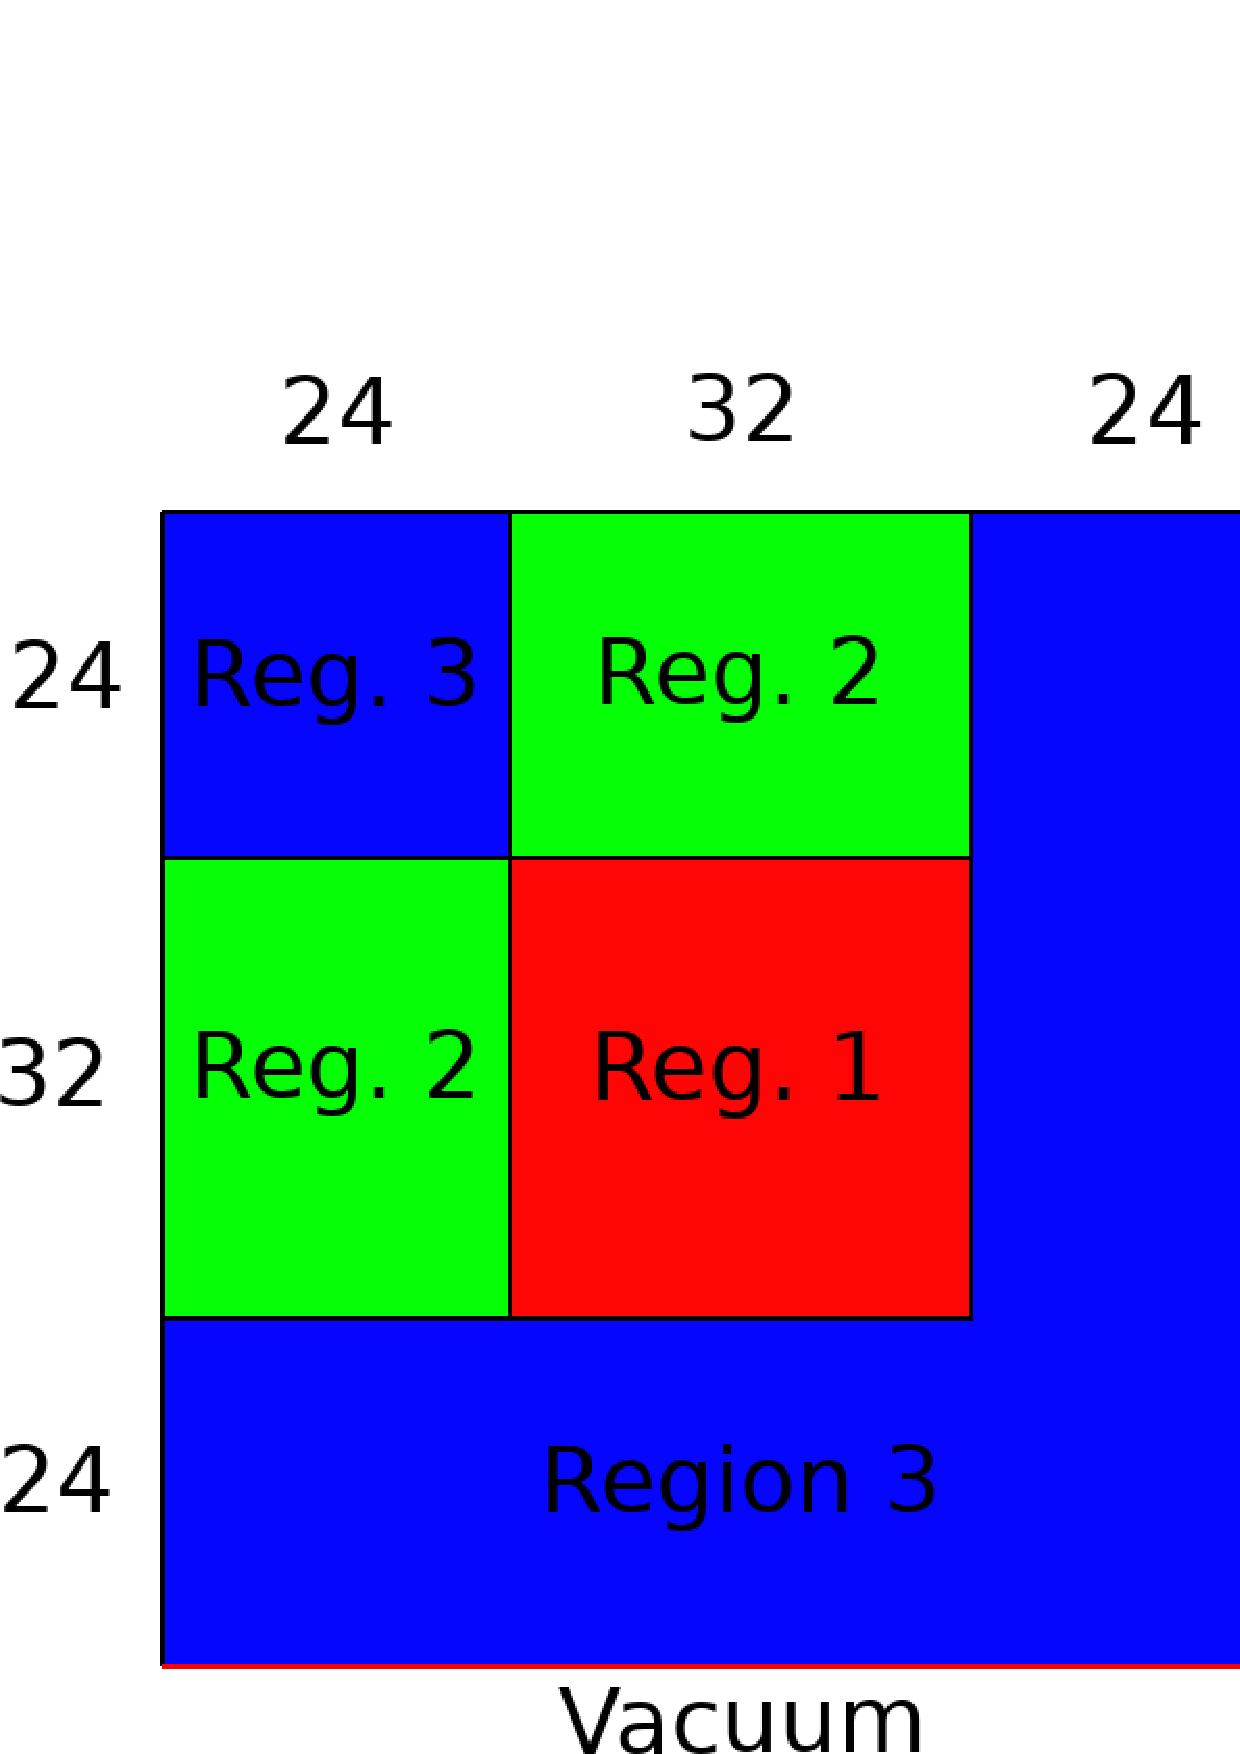
\includegraphics[width=0.5\linewidth]{twigl.png}\\
	\caption{\label{image:canonsummary}Геометрическая модель 1/4 активной зоны теста TWIGL-2D.}
	\label{ris:twigl}
\end{center}
\end{figure}

\begin{table}[htp]
\caption{\label{table:coeff}Диффузионные константы для теста TWIGL-2D.}
\label{t1}
\begin{center}
\begin{tabular}{rrrr}
\hline
Материал & 1 & 2 & 3\\
\hline 
$\Sigma_{t1}$ & 0.2481 & 0.2481 & 0.2644 \\
$\Sigma_{t2}$ & 0.9833 & 0.9833 & 0.7167 \\
$\Sigma_{a1}$ & 0.01 & 0.01 & 0.008\\
$\Sigma_{a2}$ & 0.15 & 0.15 & 0.05\\
$\Sigma_{s,1\rightarrow2}$ & 0.01 & 0.01  & 0.01\\
$\Sigma_{s,1\rightarrow1}$ & 0.2281 & 0.2281 & 0.2464\\
$\Sigma_{s,2\rightarrow2}$ & 0.8333 & 0.8333 & 0.6667\\
$\nu_1\Sigma_{f1}$ & 0.007 & 0.007 & 0.003\\
$\nu_2\Sigma_{f2}$ & 0.2 & 0.2 & 0.06\\
\hline
\end{tabular}
\end{center}
\end{table}

We define the next scenario of the process:
\begin{itemize}
\item The $\lambda$-spectral problem is solved and the solution is taken as the initial condition;
\item Calculation for the non-stationary model at the time range from 0 to 0.4 sec;
\item At $t=0.1$ sec and $t=0.3$ sec $\Sigma_a$ for fuel in the zone 1 changes to +2\% and -3\%, respectively (simulation of insertion or withdrawal of control rods).
\end{itemize}
At each time the integrated power is calculated as
\begin{equation}\label{13}
P(t) = a\int_{\Omega}\Sigma_f \phi d\bm x,
\end{equation}

where $a$ is the normalization coefficient, which corresponds to a given value of the integrated power.

В задаче представлены три сценария развития переходного процесса: возмущение скачком TWIGL-S, линейное возмущение TWIGL-R и комбинированное TWIGL-C. Все возмущения происходят в зоне 1.
Возмущение скачком инициируется посредством уменьшения теплового сечения деления $\Sigma_{a2}$ на $0.0035$ см$^{-1}$ в нулевой момент времени. 
В случае линейного возмущения $\Sigma_{a2}$ линейно уменьшается на $0.0035$ см$^{-1}$ в течение $0.2$ секунд.
Комбинированное возмущение происходит следующим образом:
$\Sigma_{a2}$ линейно уменьшается на $0.0035$ см$^{-1}$ в течении $0.2$ секунд; в момент времени $0.2$ секунд происходит скачкообразное увеличение на $0.00525$ см$^{-1}$; линейно увеличивается на $0.00175$ см$^{-1}$  с момента времени $0.2$ секунд до $0.4$ секунд;  скачкообразное уменьшение на $0.0035$ см$^{-1}$.

В комбинированном случае представлены другие параметры для запаздывающих нейтронов: $v_1 = 10^7$ см/с и $v_2 = 10^5$ см/с; эффективная доля запаздывающих нейтронов составляет $\beta = 0.0064$;  постоянная распада предшественников запаздывающих нейтронов $\lambda = 0.08$ с$^{-1}$. 
Динамическое поведение исследуется на интервале $0 \leq t \leq 0.5$ с для всех трех случаев. 

\subparagraph{Решение $\lambda$-спектральной задачи}
Результаты расчета теста TWIGL-2D приведены в таблице \ref{table:t2-lamda}.
Здесь приняты следующие обозначения: 
$k_{dif}(\gamma)$ --- эффективный коэффициент размножения по диффузионной модели для различных значений параметра альбеда; $k_{sp_3}$ --- эффективный коэффициент размножения по транспортной SP$_3$ модели. 
Представленные данные демонстрируют сходимость приближенно вычисляемых собственных значений при сгущении сетки $n$ и при увеличении степени полиномов конечных элементов $p$.
На рисунках \ref{ris:dif_pwr_0.5}, \ref{ris:dif_pwr_100}, \ref{ris:sp3_pwr} показаны расчеты нормированных мощностей (\ref{13}) для трех случаев по нодам 8х8 см. 

\begin{table}[h]
\caption{Результаты расчета $\lambda$-спектральной задачи.}
\label{table:t2-lamda}
\begin{center}
\begin{tabular}{r r r r r}
\hline
$n$ & $p$ & $k_{dif} (\gamma=0.5)$ & $k_{dif} (\gamma=100)$ & $k_{sp_3}$\\
\hline
	& 1	& 0.915519 & 0.913286 & 0.916144\\
2	& 2	& 0.915519 & 0.913333 & 0.916190\\
	& 3	& 0.915419 & 0.913234 & 0.916094\\ 
\hline
	& 1	& 0.915486 & 0.913288 & 0.916147\\
8& 2	& 0.915423 & 0.913238 & 0.916096\\
	& 3	& 0.915408 & 0.913223 & 0.916076\\ 
\hline
	& 1	& 0.915434 & 0.913245 & 0.916102\\
32& 2	& 0.915409 & 0.913223 & 0.916076\\
	& 3	& 0.915408 & 0.913222 & 0.916073\\
\hline
\end{tabular}
\end{center}
\end{table}

\begin{figure}[ht]
\begin{center}
	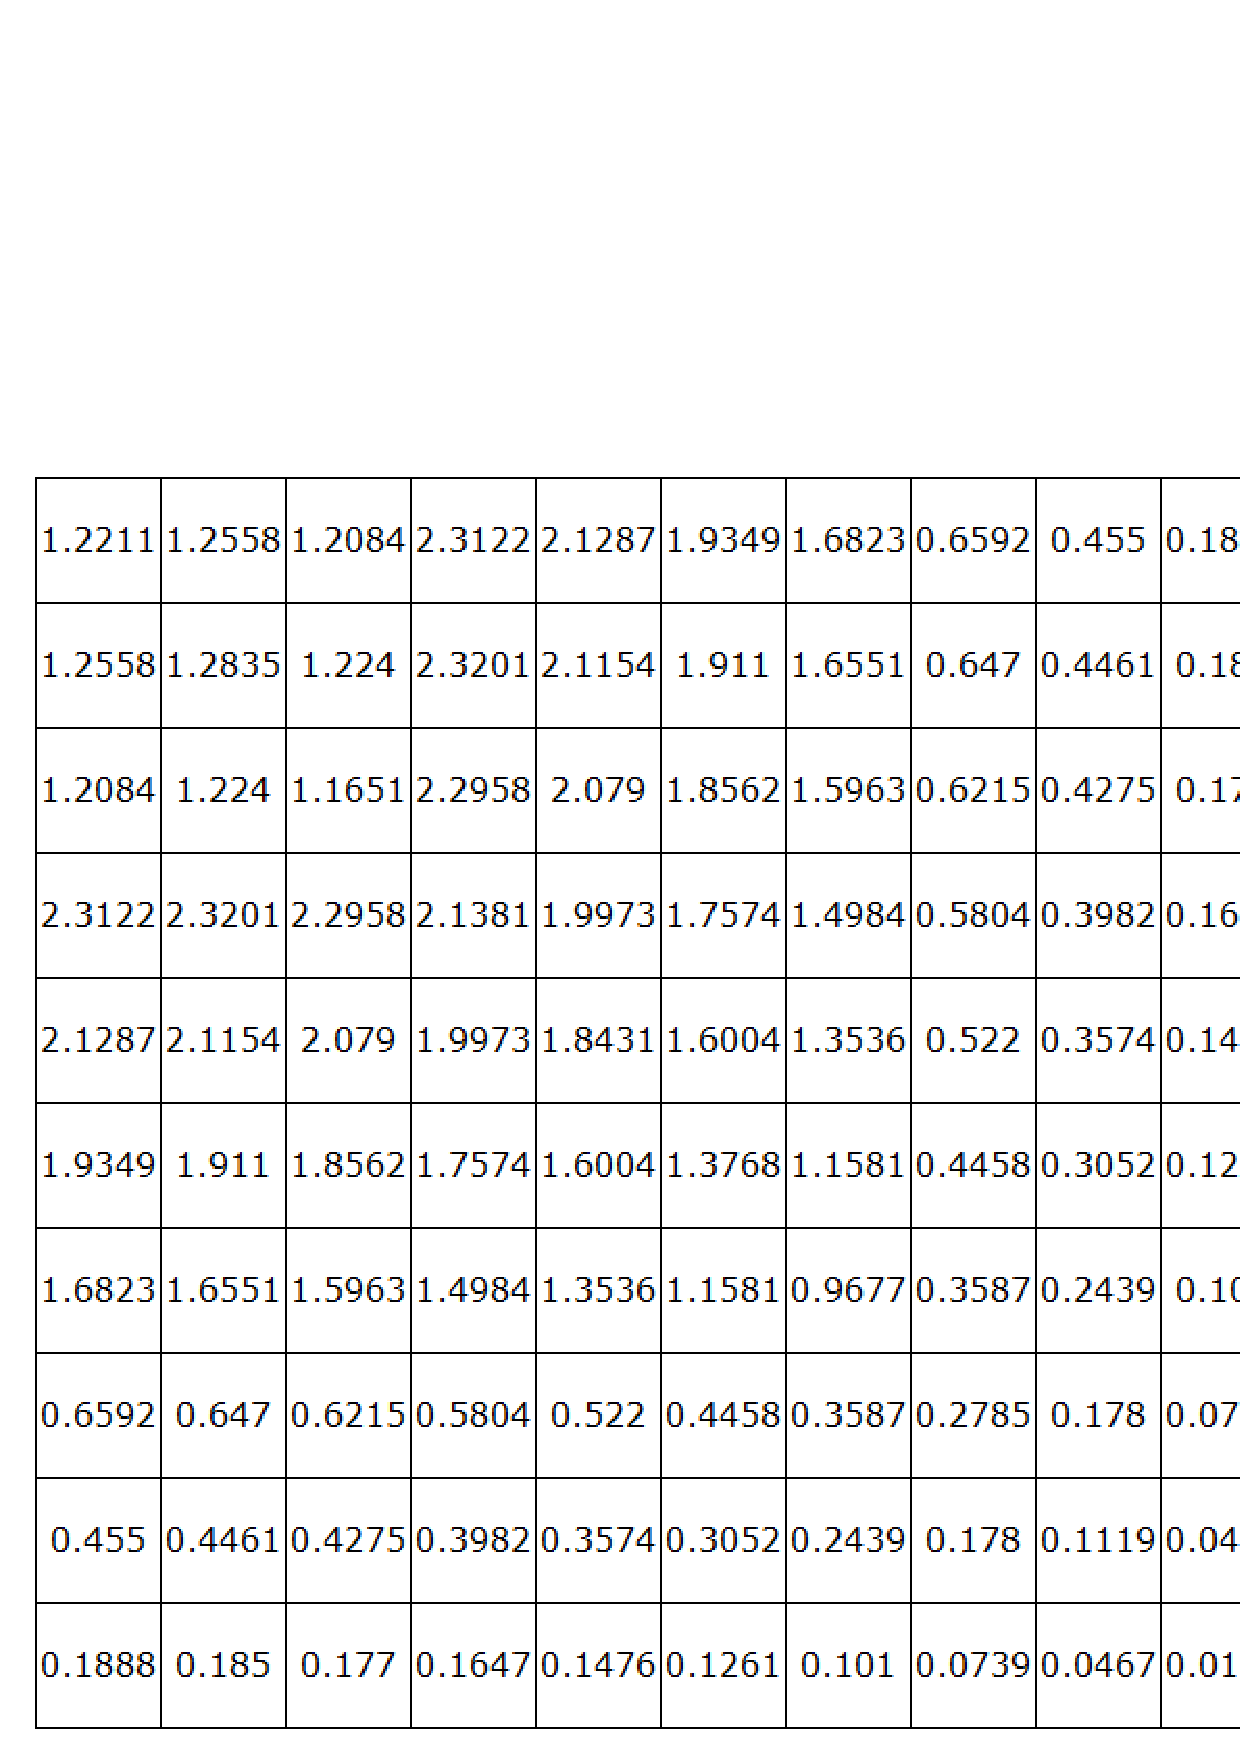
\includegraphics[width=0.5\linewidth]{dif_pwr.png}\\
	\caption{\label{image:canonsummary} Нормированная мощность по диффузионной модели при $\gamma=0.5$.}
	\label{ris:dif_pwr_0.5}
\end{center}
\end{figure}

\begin{figure}[ht]
\begin{center}
	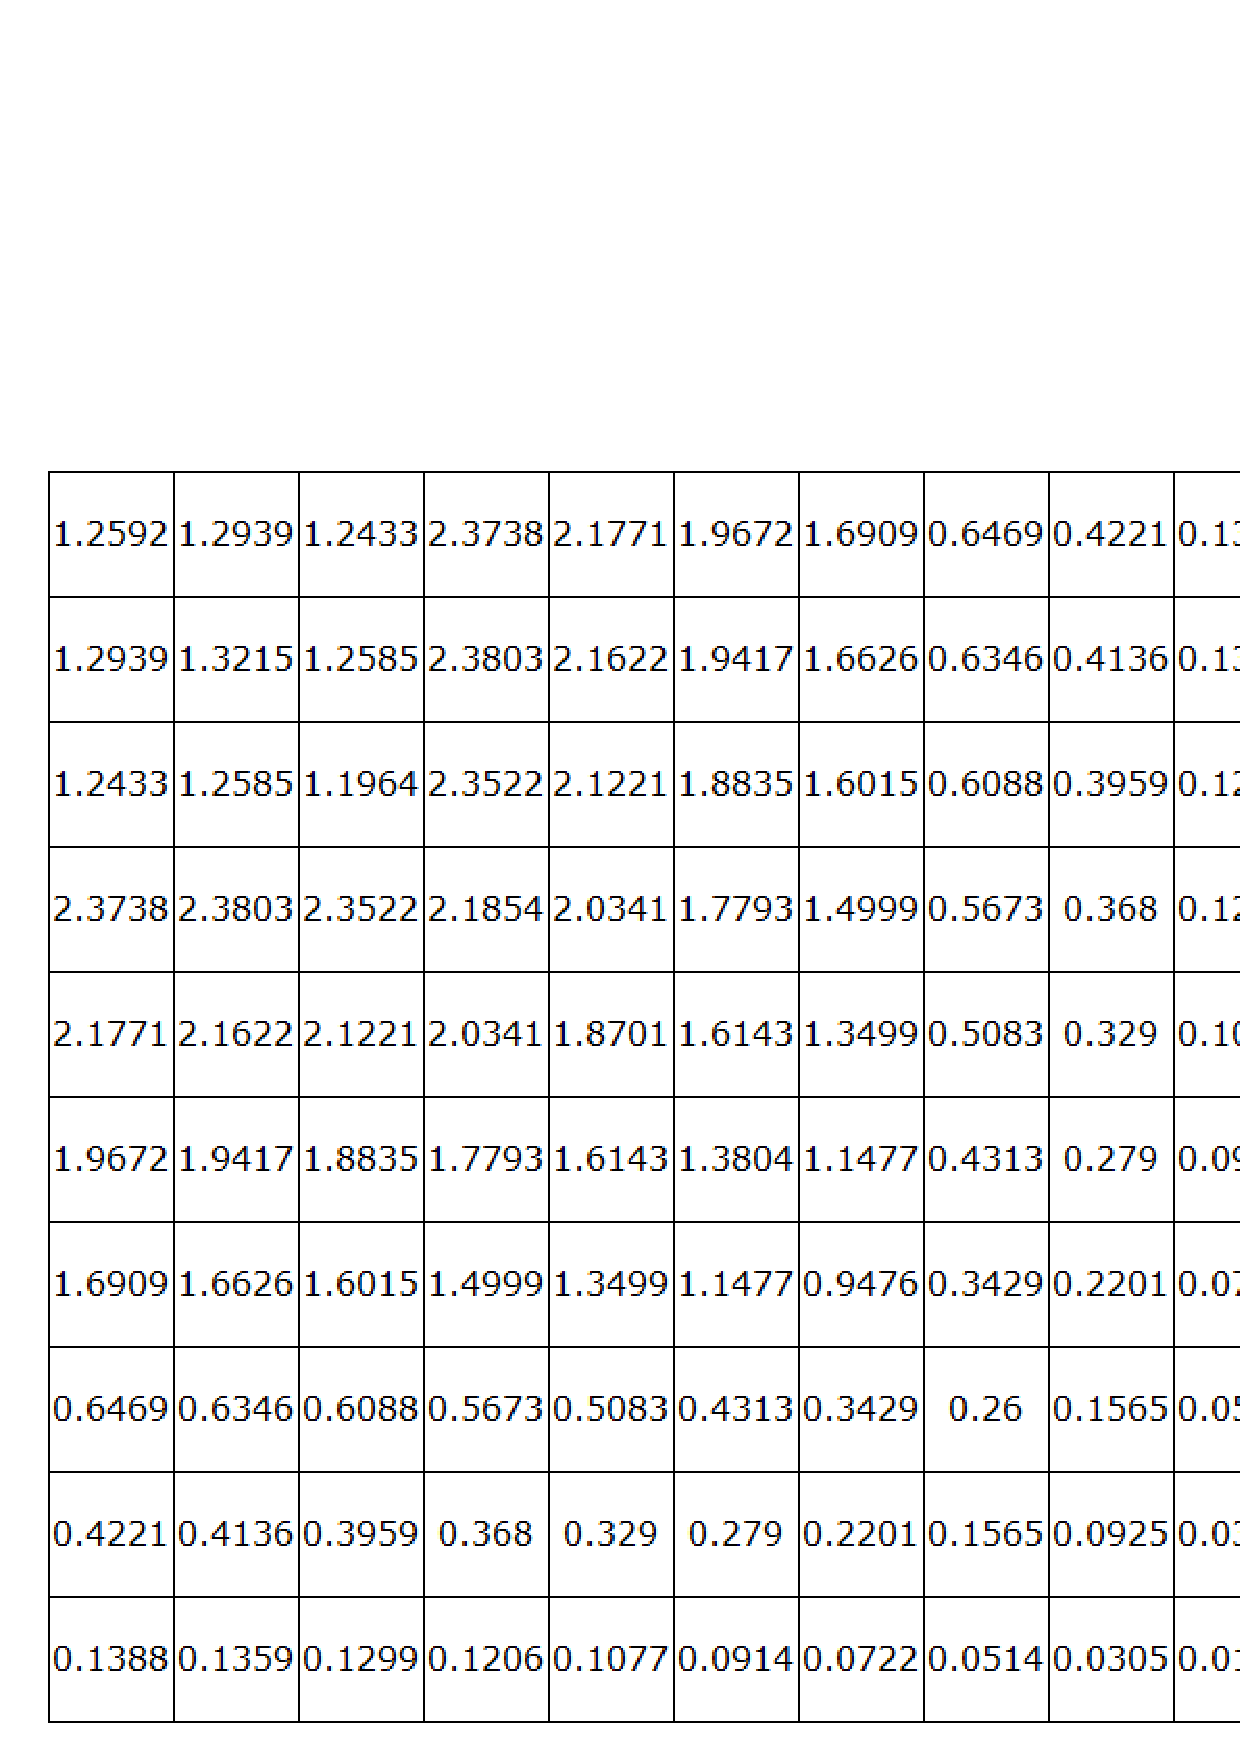
\includegraphics[width=0.5\linewidth]{dif_pwr_100.png}\\
	\caption{\label{image:canonsummary} Нормированная мощность по диффузионной модели при $\gamma=100$.}
	\label{ris:dif_pwr_100}
\end{center}
\end{figure}

\begin{figure}[ht]
\begin{center}
	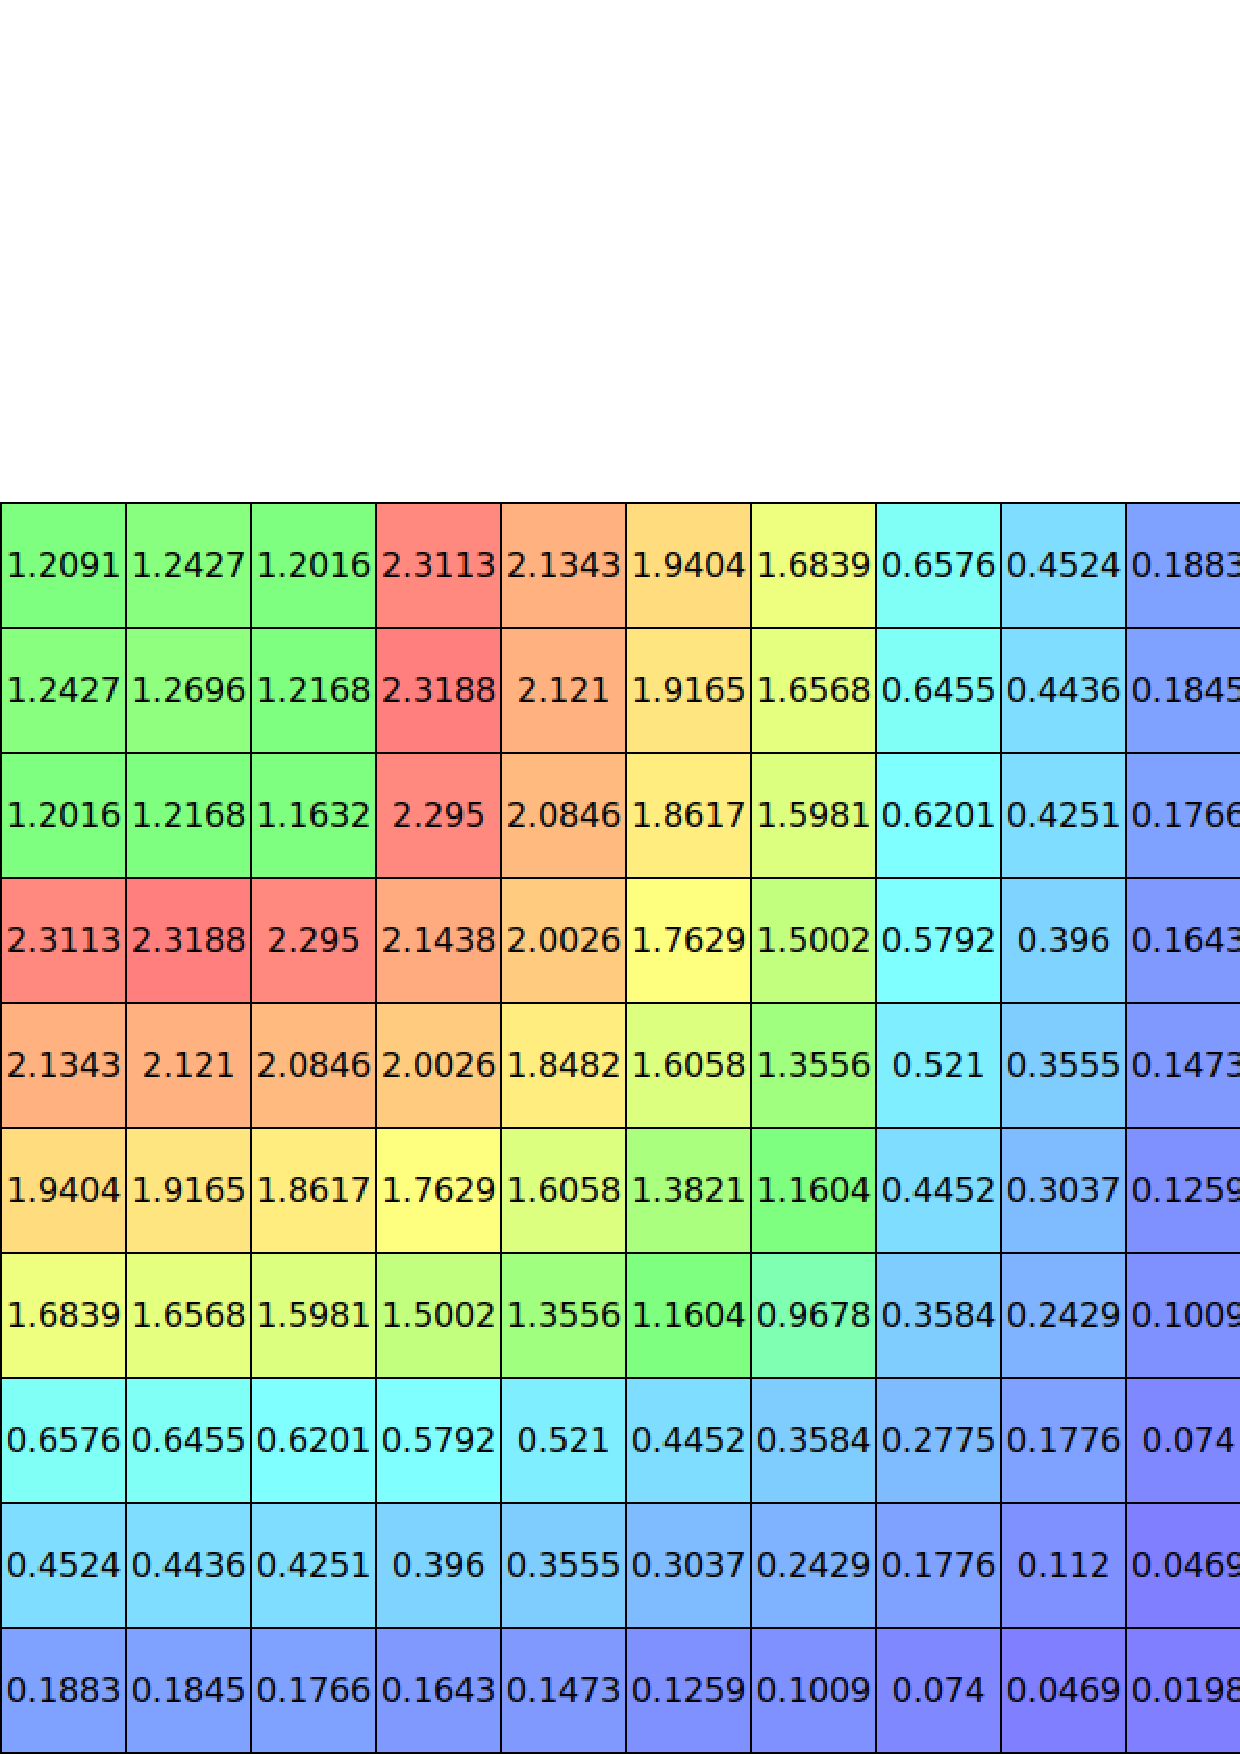
\includegraphics[width=0.5\linewidth]{sp3_pwr.png}\\
	\caption{\label{image:canonsummary} Нормированная мощность по транспортной $SP_3$ модели.}
	\label{ris:sp3_pwr}
\end{center}
\end{figure}

\subparagraph{Решение нестационарной задачи}
Представлены исследования различных шагов по времени для всех трех сценариев.  В качестве сетки по пространству взят вариант при $n=36,\ p=2$, а для эталонного решения взяты результаты на мелкой сетке $n=144,\ p=3,\ \tau=1$ мс.

\subparagraph{Сценарий №1}
В таблице \ref{table:twigl-s} представлены результаты эталонных решений TWIGL-S при $n=32, p=3, \tau=1$ мс по диффузионной и транспортной моделях.
На рисунке \ref{ris:sp3_ref_s} показано эталонное решение TWIGL-S по транспортной модели, а на рисунке \ref{ris:odds_s} показаны различия диффузионных эталонных решений относительно транспортного эталонного решения. 
Далее, на рисунках \ref{ris:dif_tau_s_0.5}, \ref{ris:dif_tau_s_100}, \ref{ris:sp3_tau_s} показаны отличия при различных шагах по времени относительно эталонных решений.

\begin{table}[ht]
\caption{Различие результатов диффузионного и транспортного расчетов для TWIGL-S.}
\label{table:twigl-s}
\begin{center}
\begin{tabular}{r r r r}
\hline
$t$ & Dif ($\gamma=0.5$) & Dif ($\gamma=100$) & SP$_3$\\
\hline
0.0 & 1.0000 & 1.0000 & 1.0000\\
0.1 & 2.0783  & 2.0613 & 2.0898\\
0.2 & 2.0961 & 2.0786 & 2.1079\\
0.3 & 2.1139 & 2.0959 & 2.1260\\
0.4 & 2.1319 & 2.1135 & 2.1442\\
0.5 & 2.1500 & 2.1311 & 2.1626\\
\hline
\end{tabular}
\end{center}
\end{table}

\begin{figure}[ht]
\begin{center}
	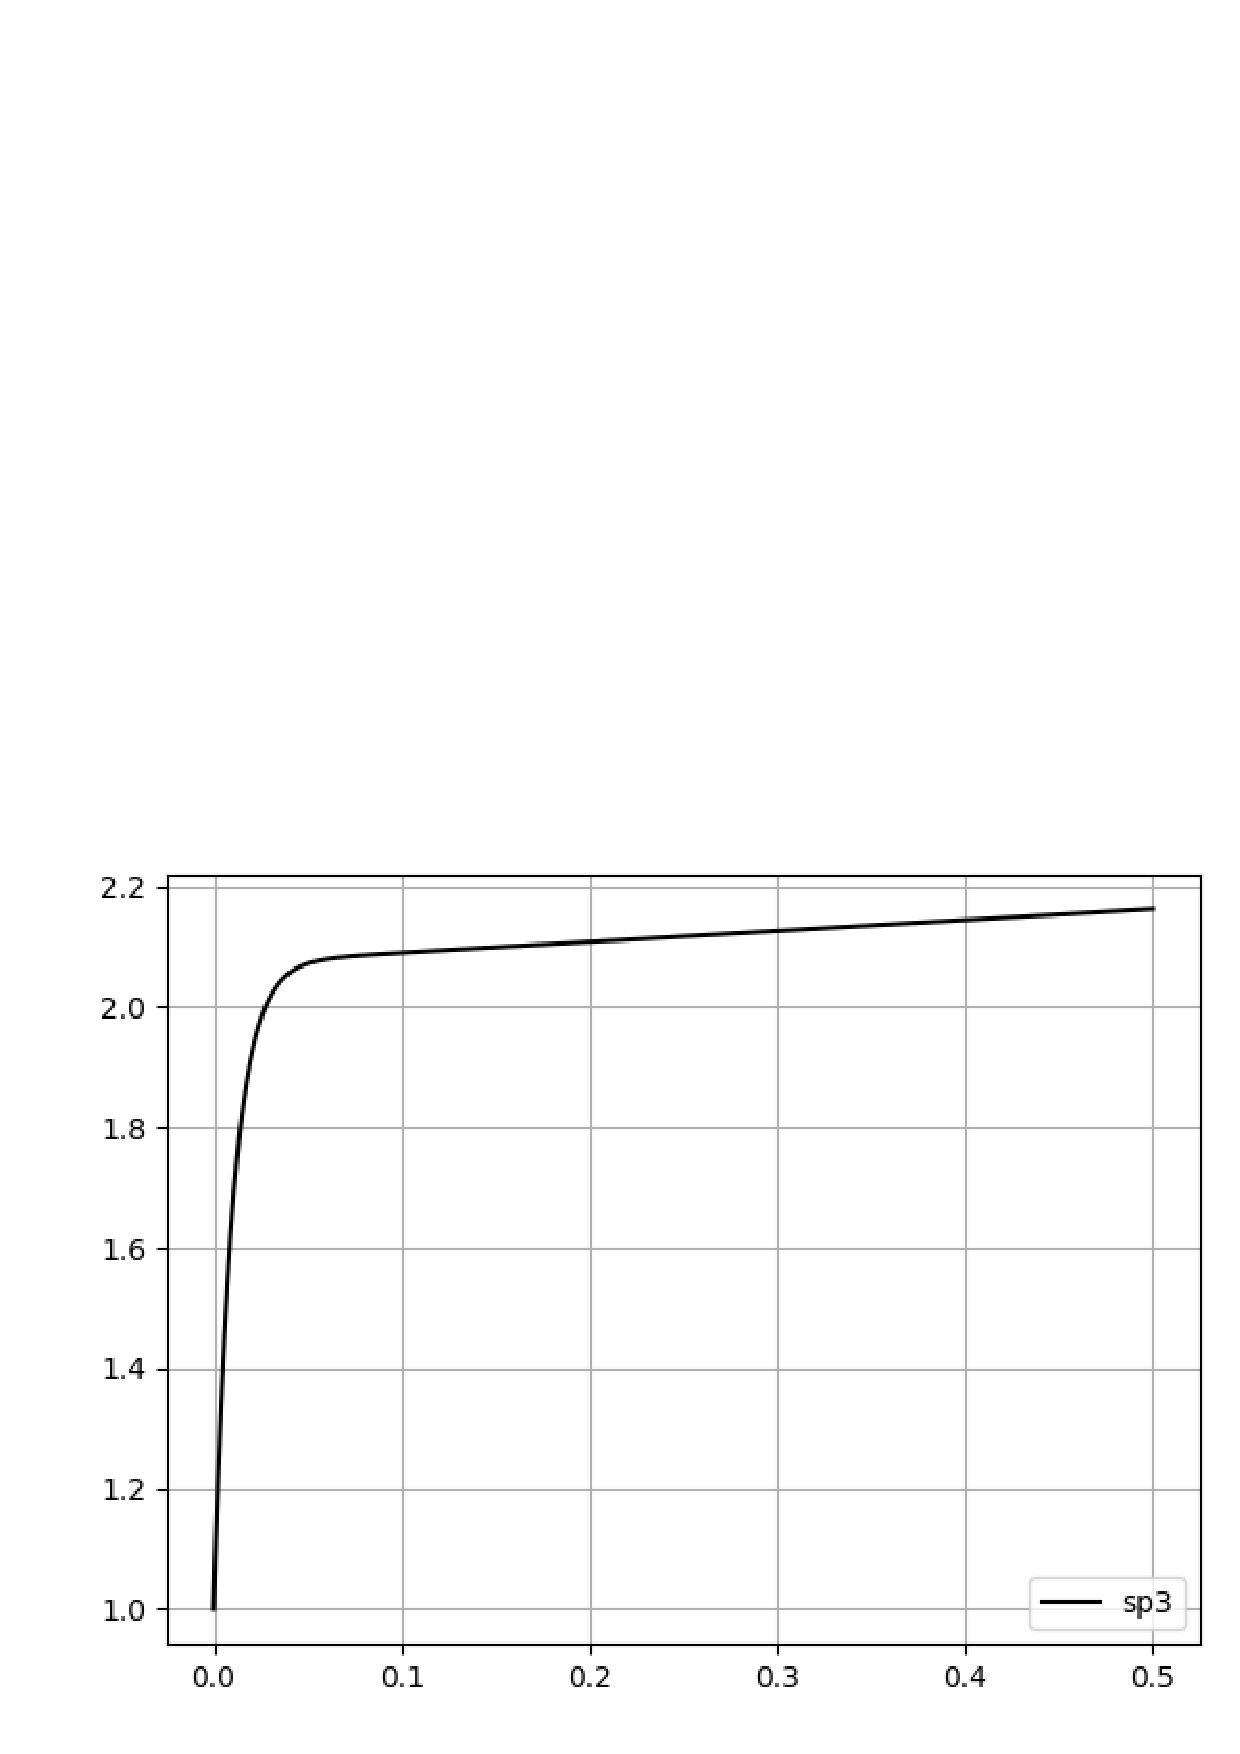
\includegraphics[width=0.5\linewidth]{sp3_ref_s.png}\\
	\caption{\label{image:canonsummary} Эталонное решение TWIGL-S по транспортной SP$_3$ модели.}
	\label{ris:sp3_ref_s}
\end{center}
\end{figure}

\begin{figure}[ht]
\begin{center}
	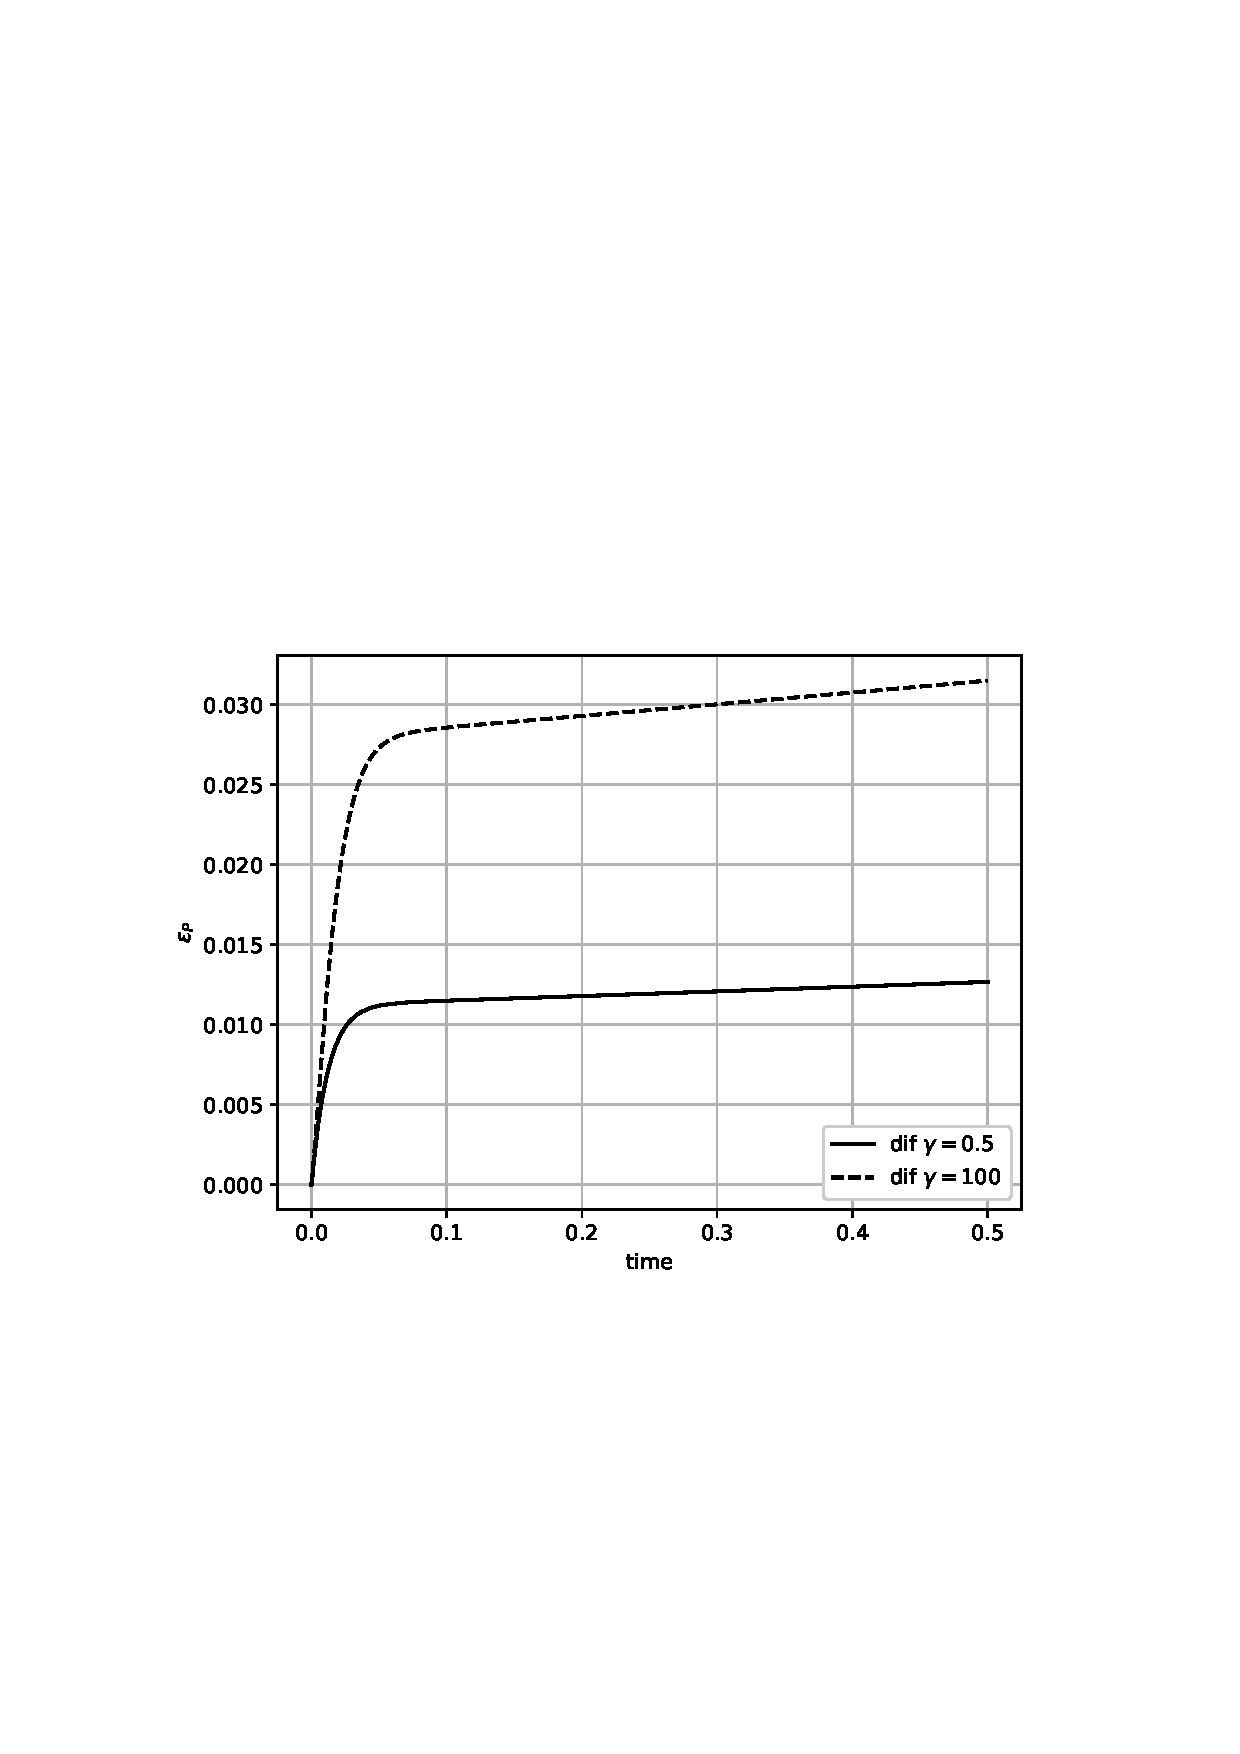
\includegraphics[width=0.5\linewidth]{odds_s.png}\\
	\caption{\label{image:canonsummary} Различия решения TWIGL-S по диффузионной модели от транспортной модели.}
	\label{ris:odds_s}
\end{center}
\end{figure}

\begin{figure}[ht]
\begin{center}
	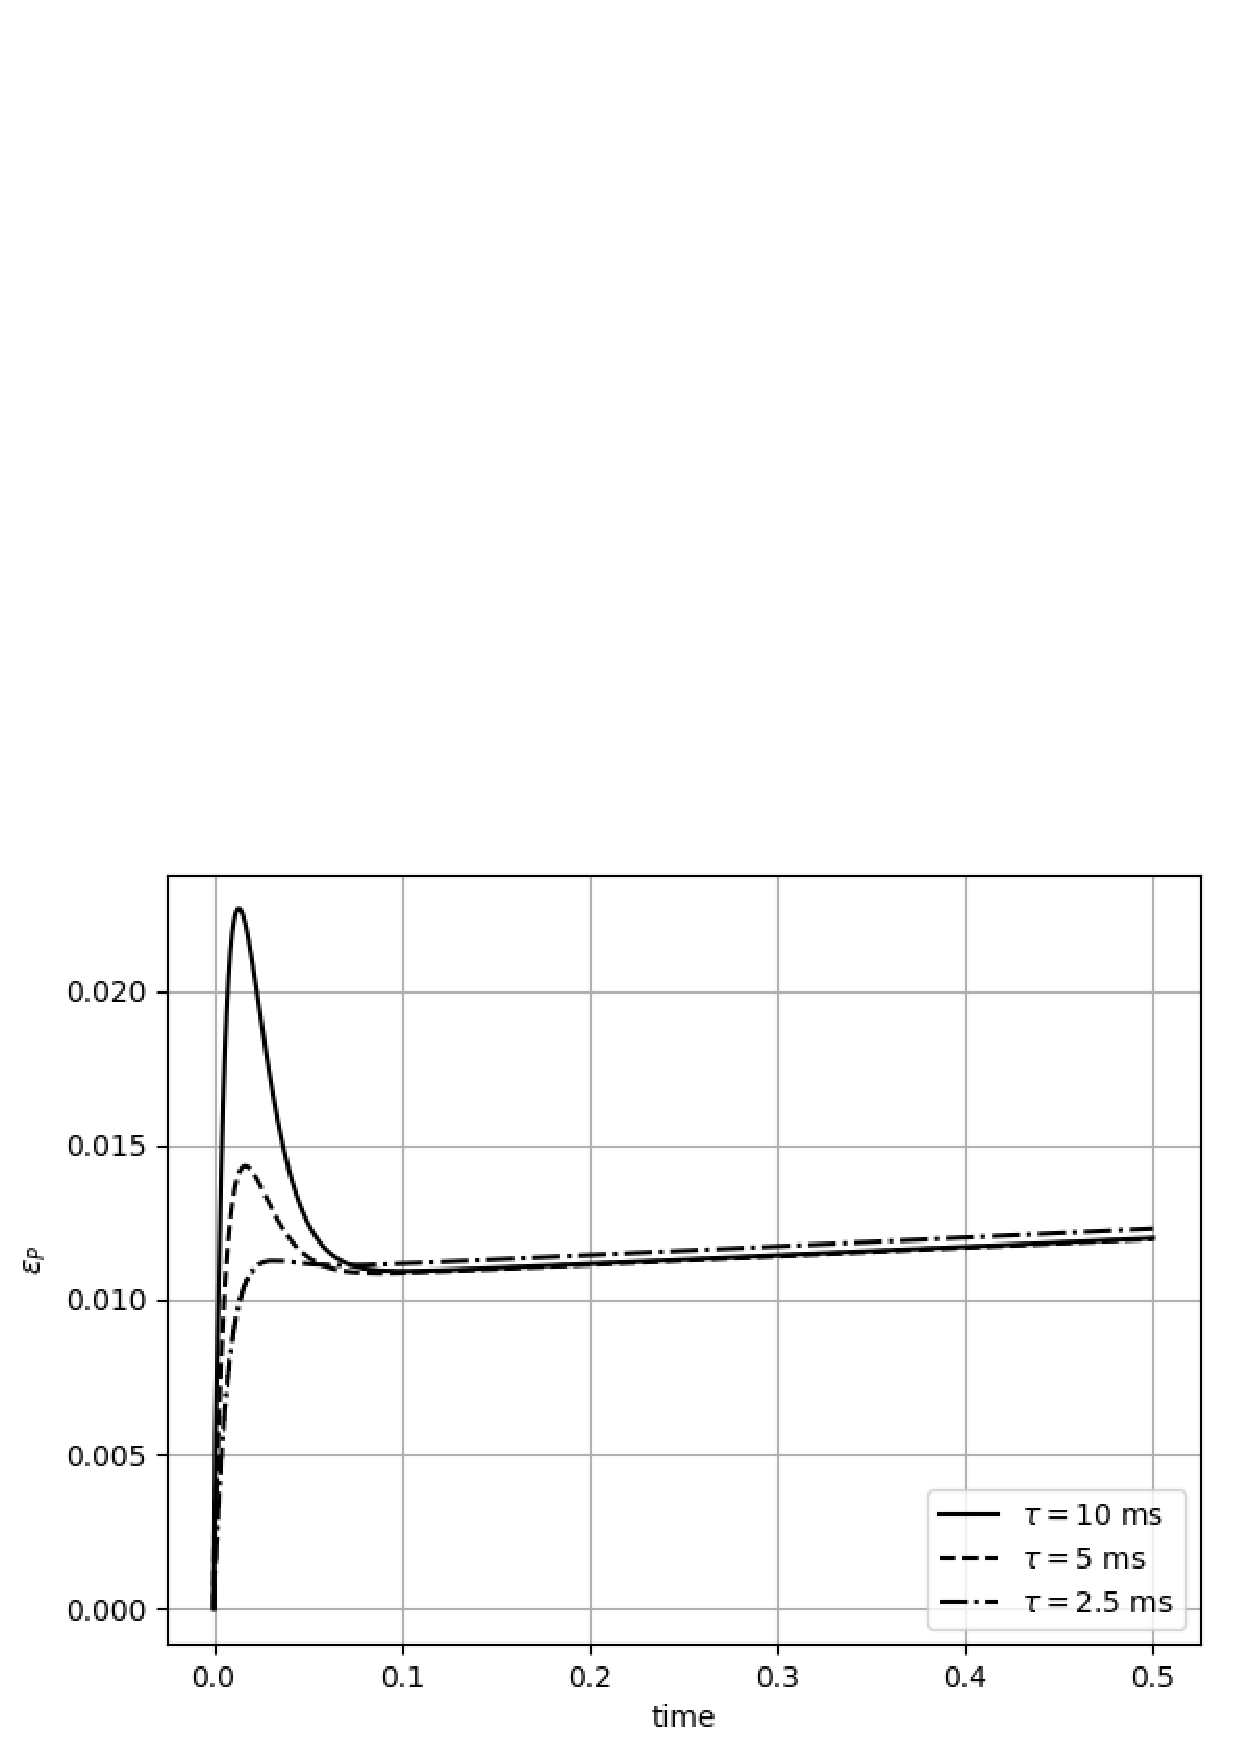
\includegraphics[width=0.45\linewidth]{dif_tau_s.png}
	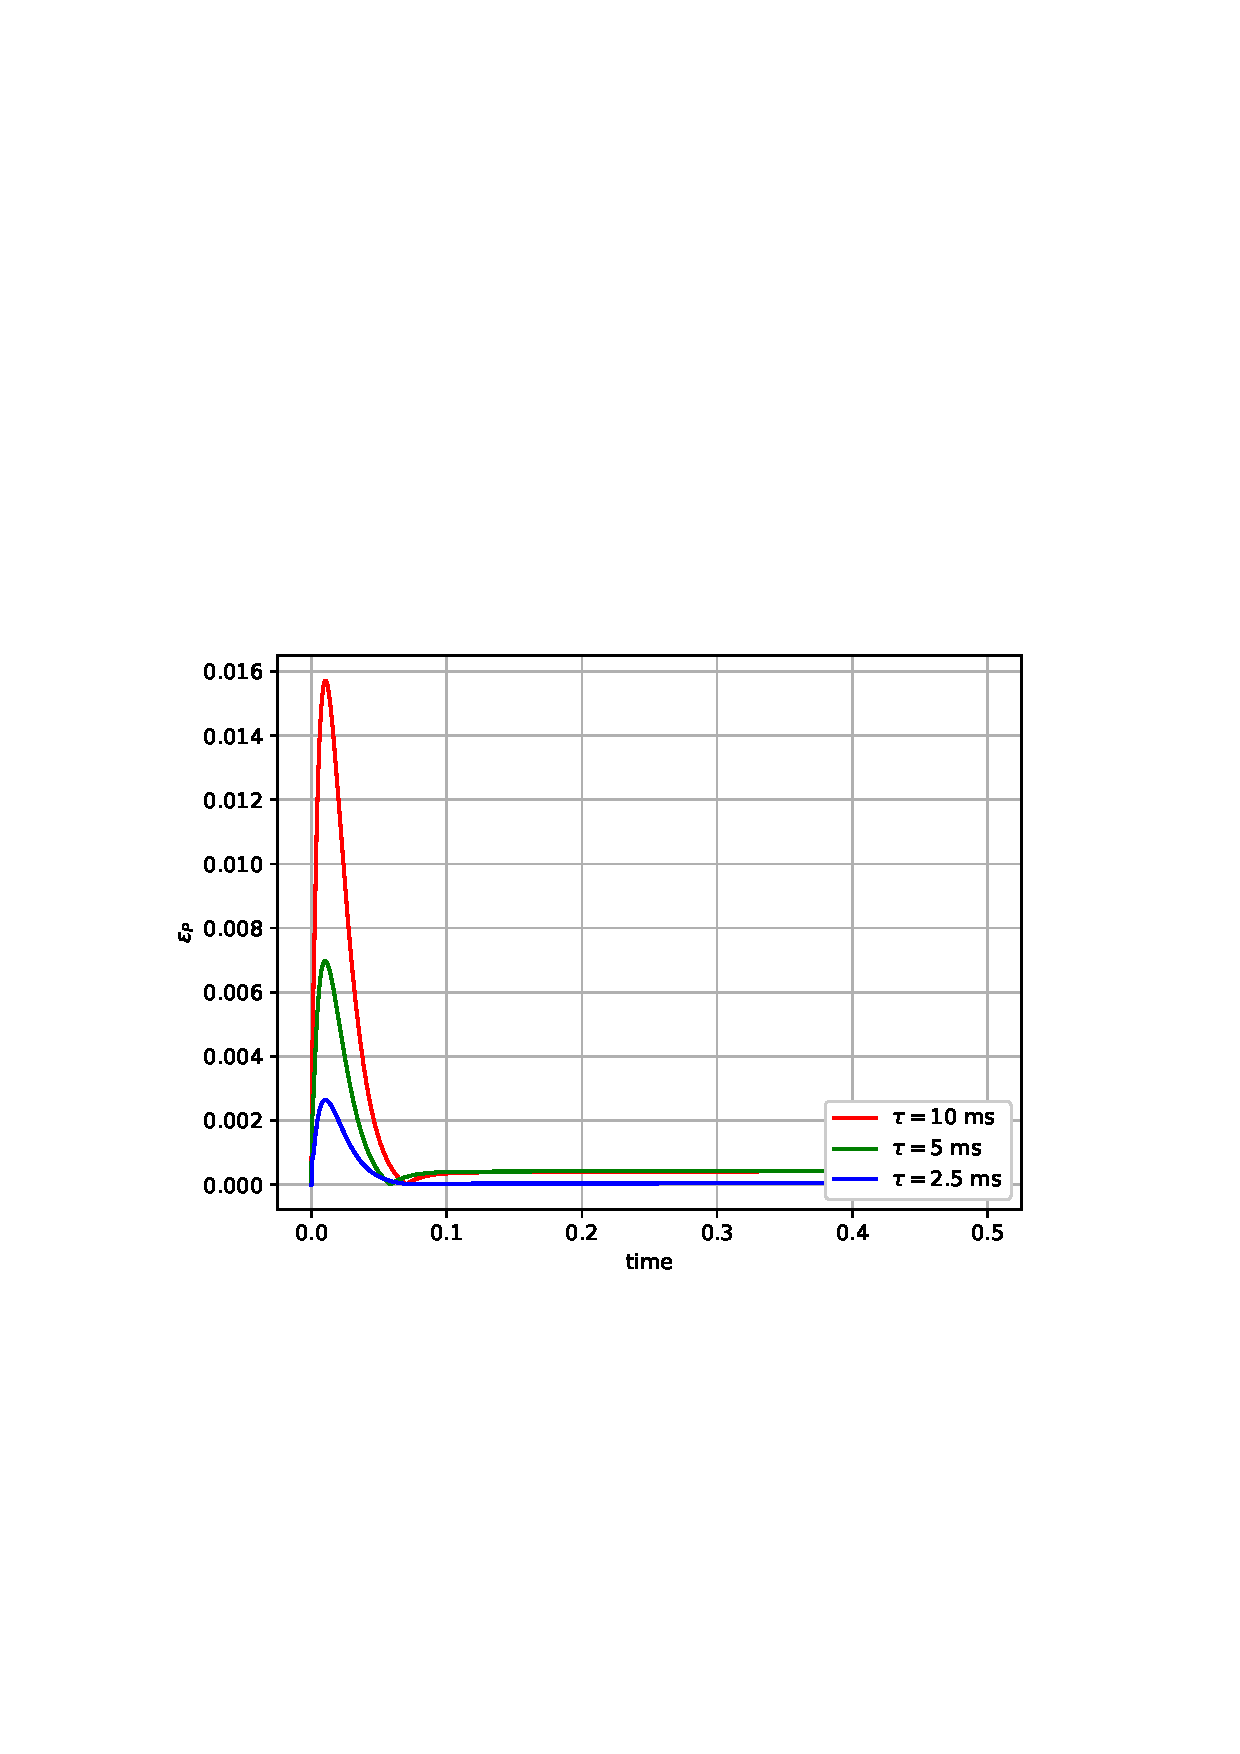
\includegraphics[width=0.45\linewidth]{dif_tau_s_100.png}\\
	\caption{\label{image:canonsummary} Результаты расчета TWIGL-S для различных шагов по времени по диффузионной модели при $\gamma=0.5$ (справа) и $\gamma=100$ (слева).}
	\label{ris:dif_tau_s_0.5}
\end{center}
\end{figure}

%\begin{figure}[ht]
%\begin{center}
%	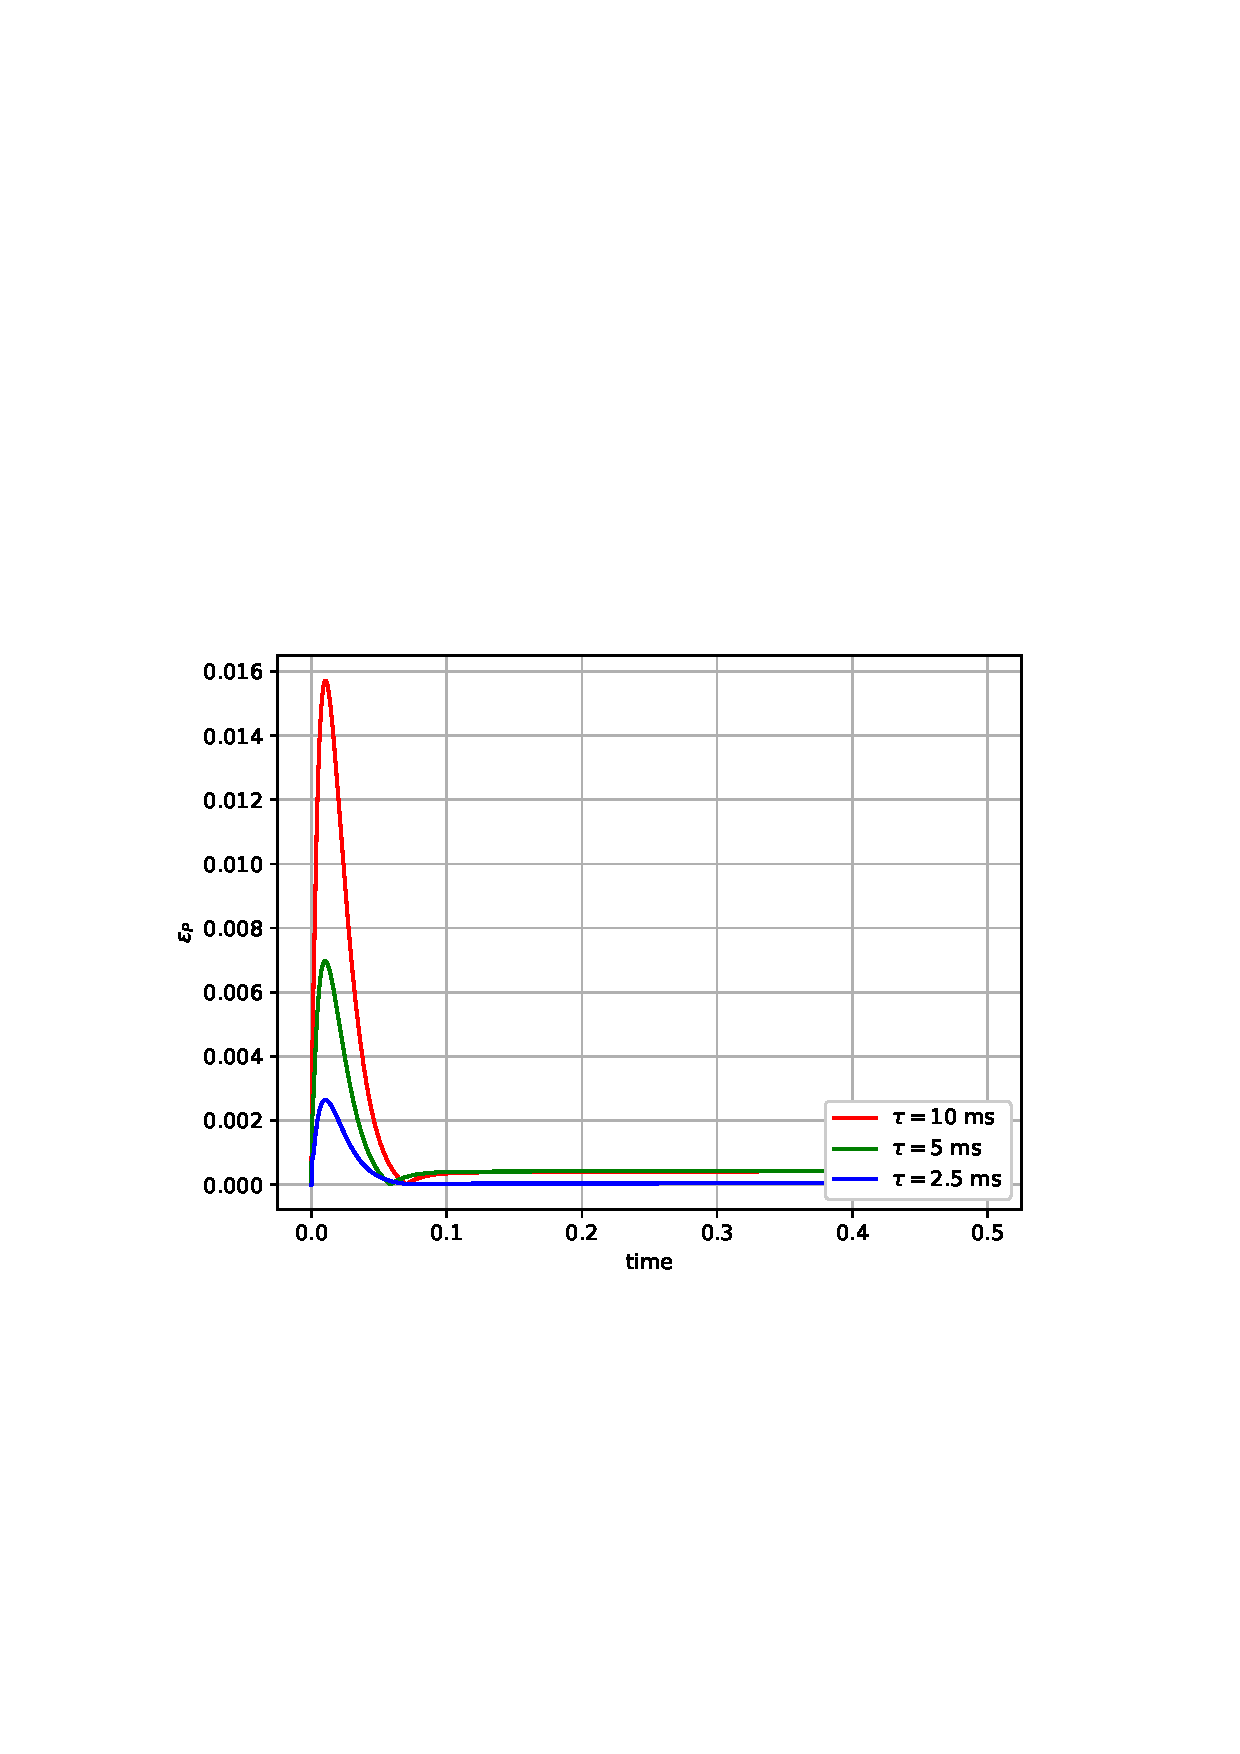
\includegraphics[width=0.5\linewidth]{dif_tau_s_100.png}\\
%	\caption{\label{image:canonsummary} Результаты расчета TWIGL-S для различных шагов по времени по диффузионной модели при $\gamma=100$.}
%	\label{ris:dif_tau_s_100}
%\end{center}
%\end{figure}

\begin{figure}[ht]
\begin{center}
	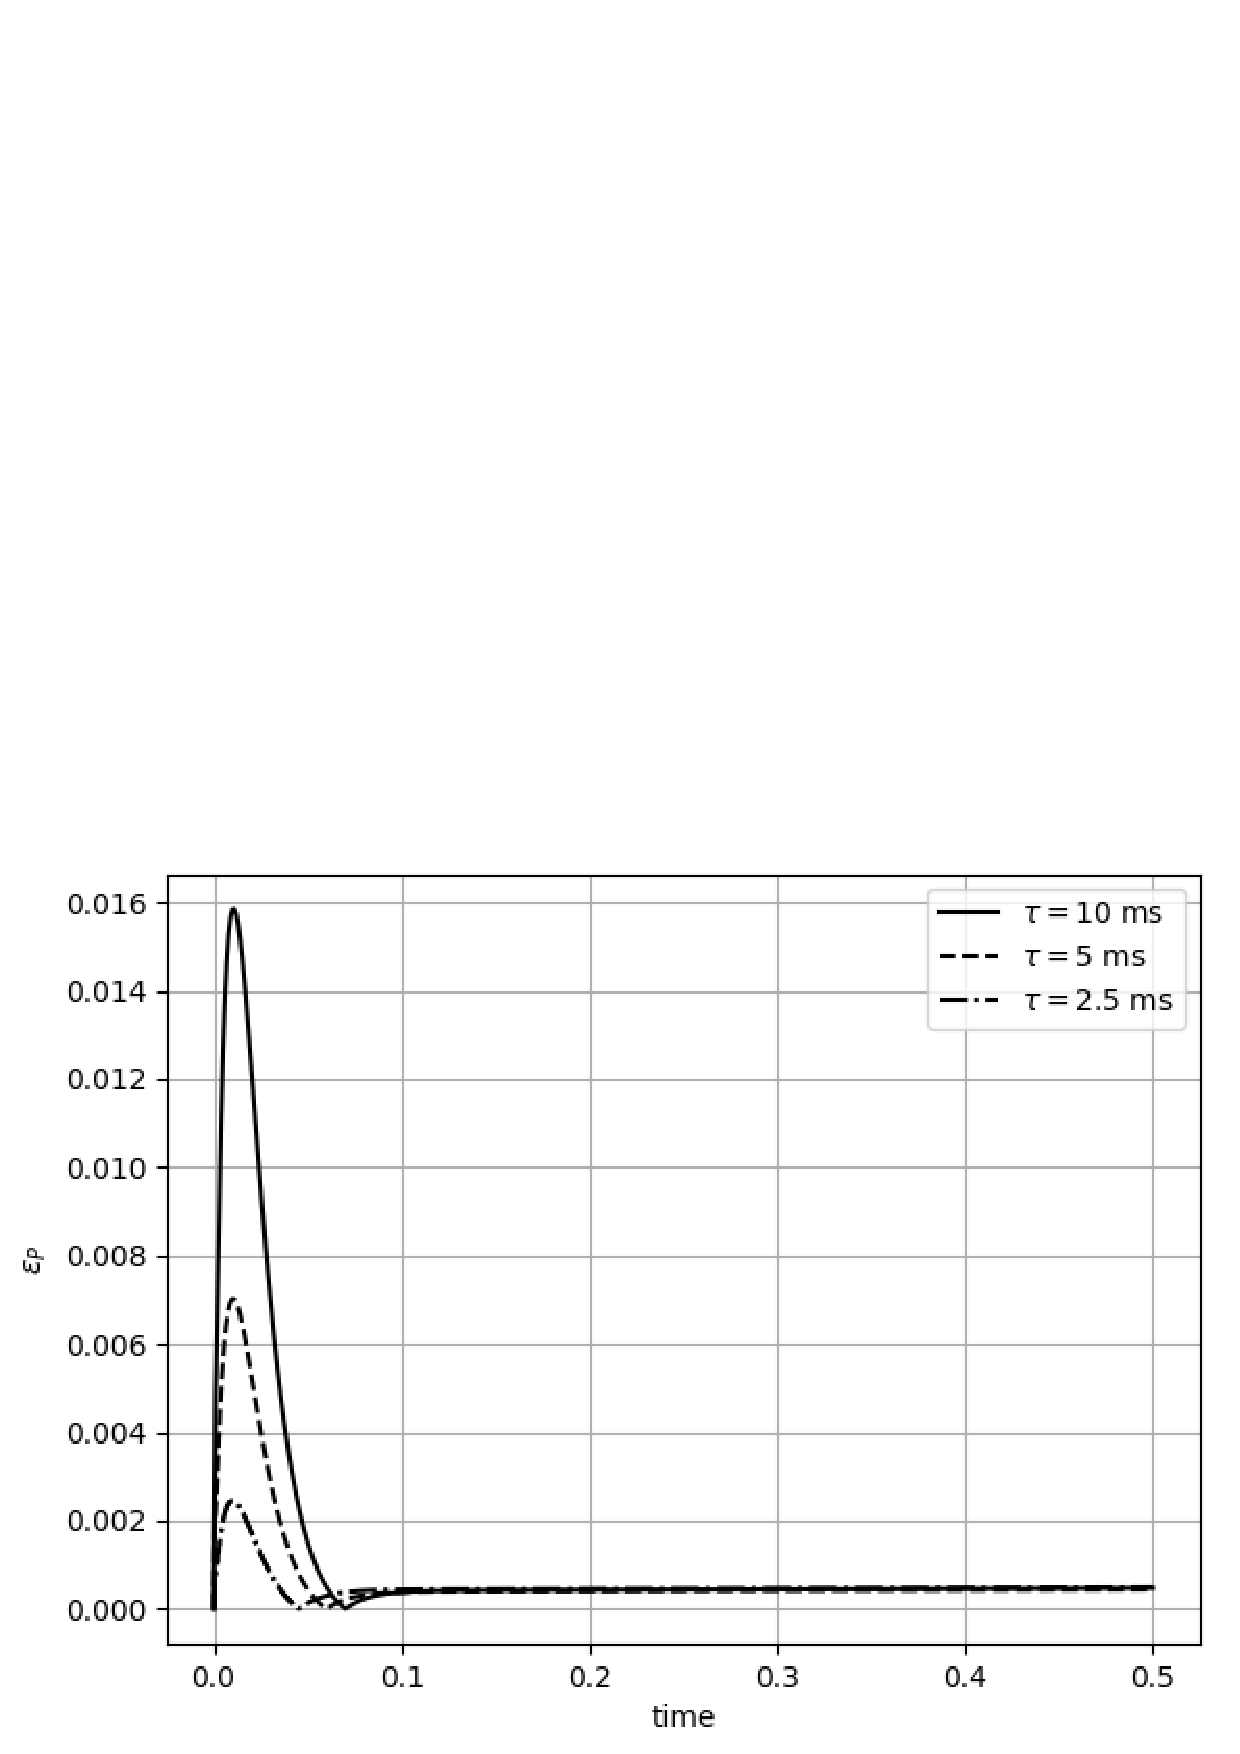
\includegraphics[width=0.5\linewidth]{sp3_tau_s.png}\\
	\caption{\label{image:canonsummary} Результаты расчета TWIGL-S для различных шагов по времени по транспортной sp3 модели.}
	\label{ris:sp3_tau_s}
\end{center}
\end{figure}

\pagebreak
\newpage

\subparagraph{Cценарий №2}
В таблице \ref{table:twigl-r} представлены результаты эталонных решений TWIGL-R при $n=32, p=3, \tau=1$ мс по диффузионной и транспортной моделях.
На рисунке \ref{ris:sp3_ref_r} показано эталонное решение TWIGL-R по транспортной модели, а на рисунке \ref{ris:odds_r} показаны различия диффузионных эталонных решений относительно транспортного эталонного решения. 
Далее, на рисунках \ref{ris:dif_tau_r_0.5}, \ref{ris:dif_tau_r_100}, \ref{ris:sp3_tau_r} показаны отличия при различных шагах по времени относительно эталонных решений.

\begin{table}[ht]
\caption{Различие результатов диффузионного и транспортного расчетов для TWIGL-R.}
\label{table:twigl-r}
\begin{center}
\begin{tabular}{r r r r}
\hline
$t$ & Dif ($\gamma=0.5$) & Dif ($\gamma=100$) & SP$_3$\\
\hline
0.0 & 1.0000 & 1.0000 & 1.0000\\
0.1 & 1.3112  & 1.3083 & 1.3134\\
0.2 & 1.9729 & 1.9595 & 1.9826\\
0.3 & 2.0921 & 2.0747 & 2.1038\\
0.4 & 2.1099 & 2.0921 & 2.1219\\
0.5 & 2.1278 & 2.1096 & 2.1401\\
\hline
\end{tabular}
\end{center}
\end{table}

\begin{figure}[ht]
\begin{center}
	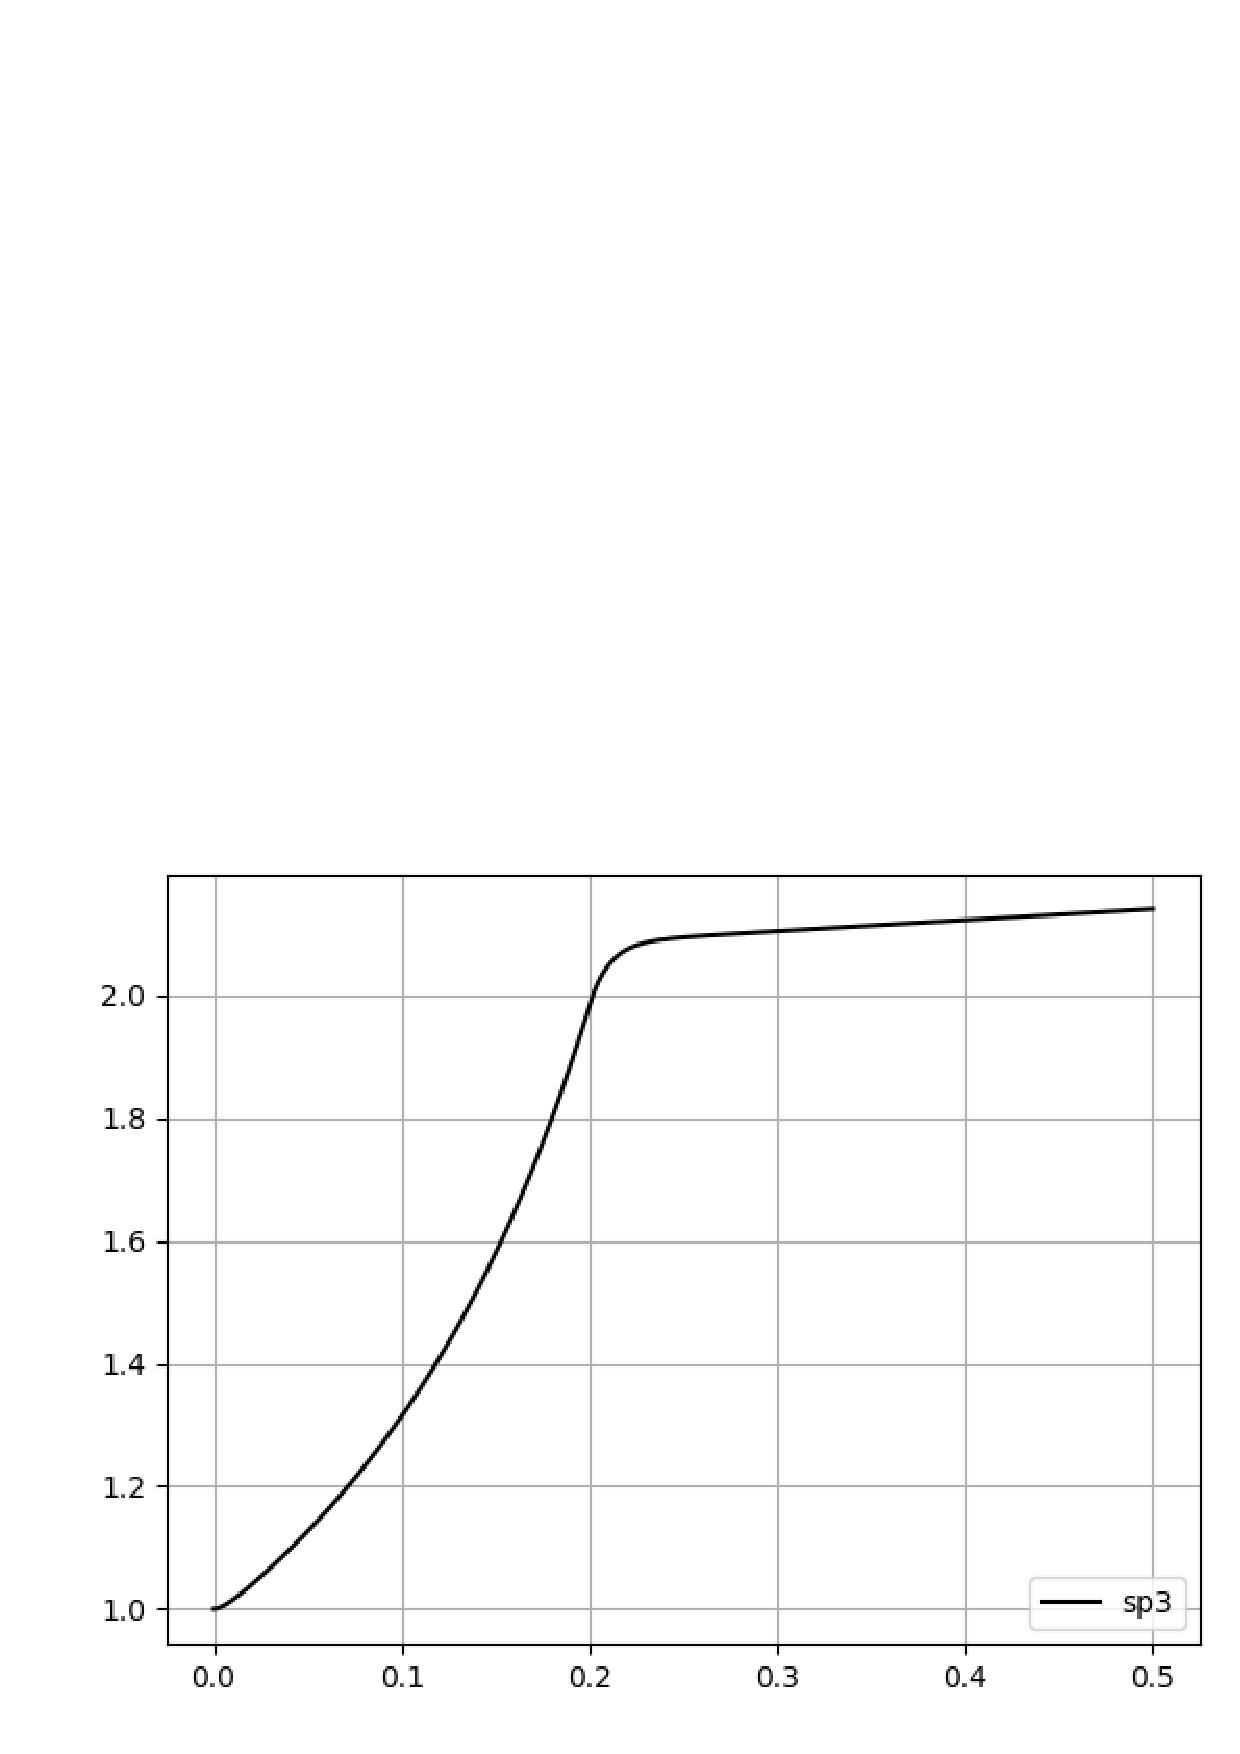
\includegraphics[width=0.5\linewidth]{sp3_ref_r.png}\\
	\caption{\label{image:canonsummary} Эталонное решение TWIGL-R по транспортной SP$_3$ модели.}
	\label{ris:sp3_ref_r}
\end{center}
\end{figure}

\begin{figure}[ht]
\begin{center}
	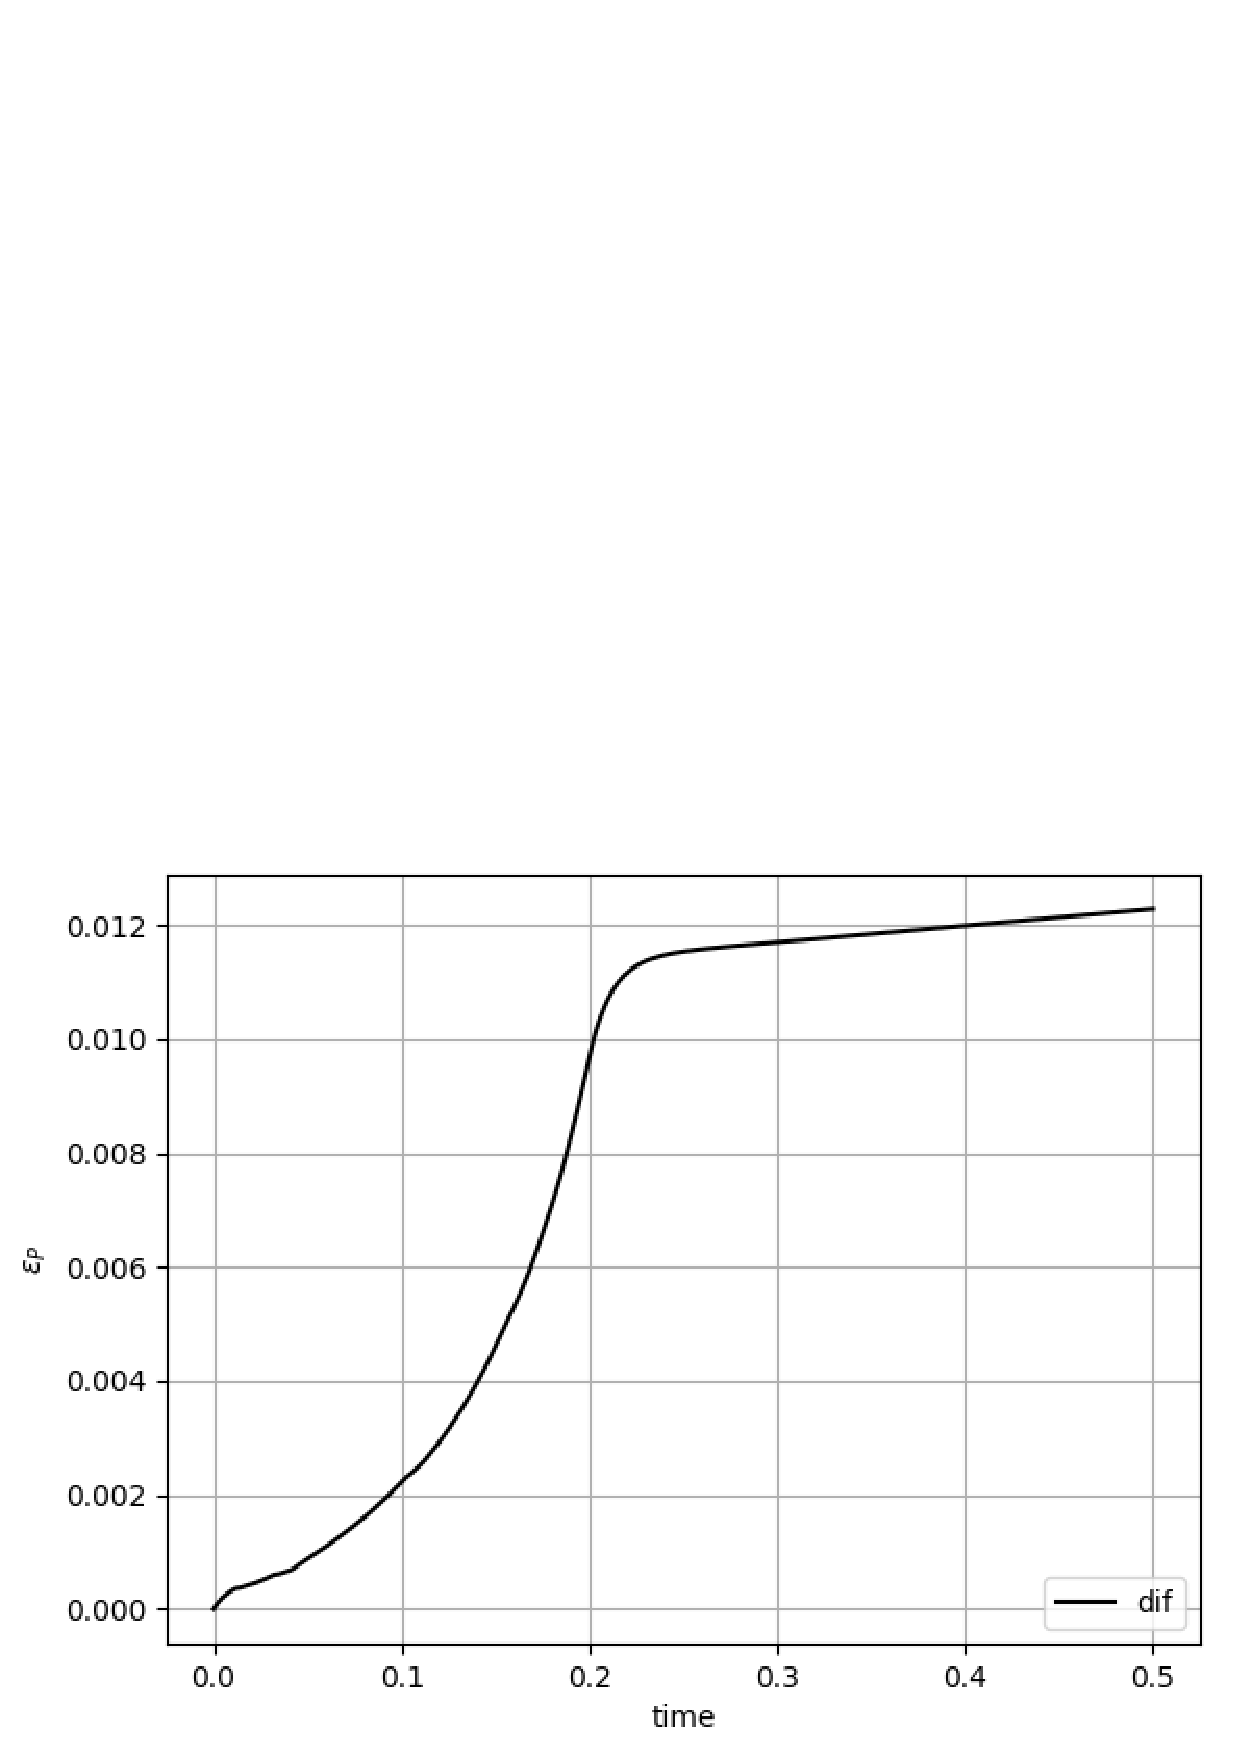
\includegraphics[width=0.5\linewidth]{odds_r.png}\\
	\caption{\label{image:canonsummary} Различия решения TWIGL-R по диффузионной модели от транспортной модели.}
	\label{ris:odds_r}
\end{center}
\end{figure}

\begin{figure}[ht]
\begin{center}
	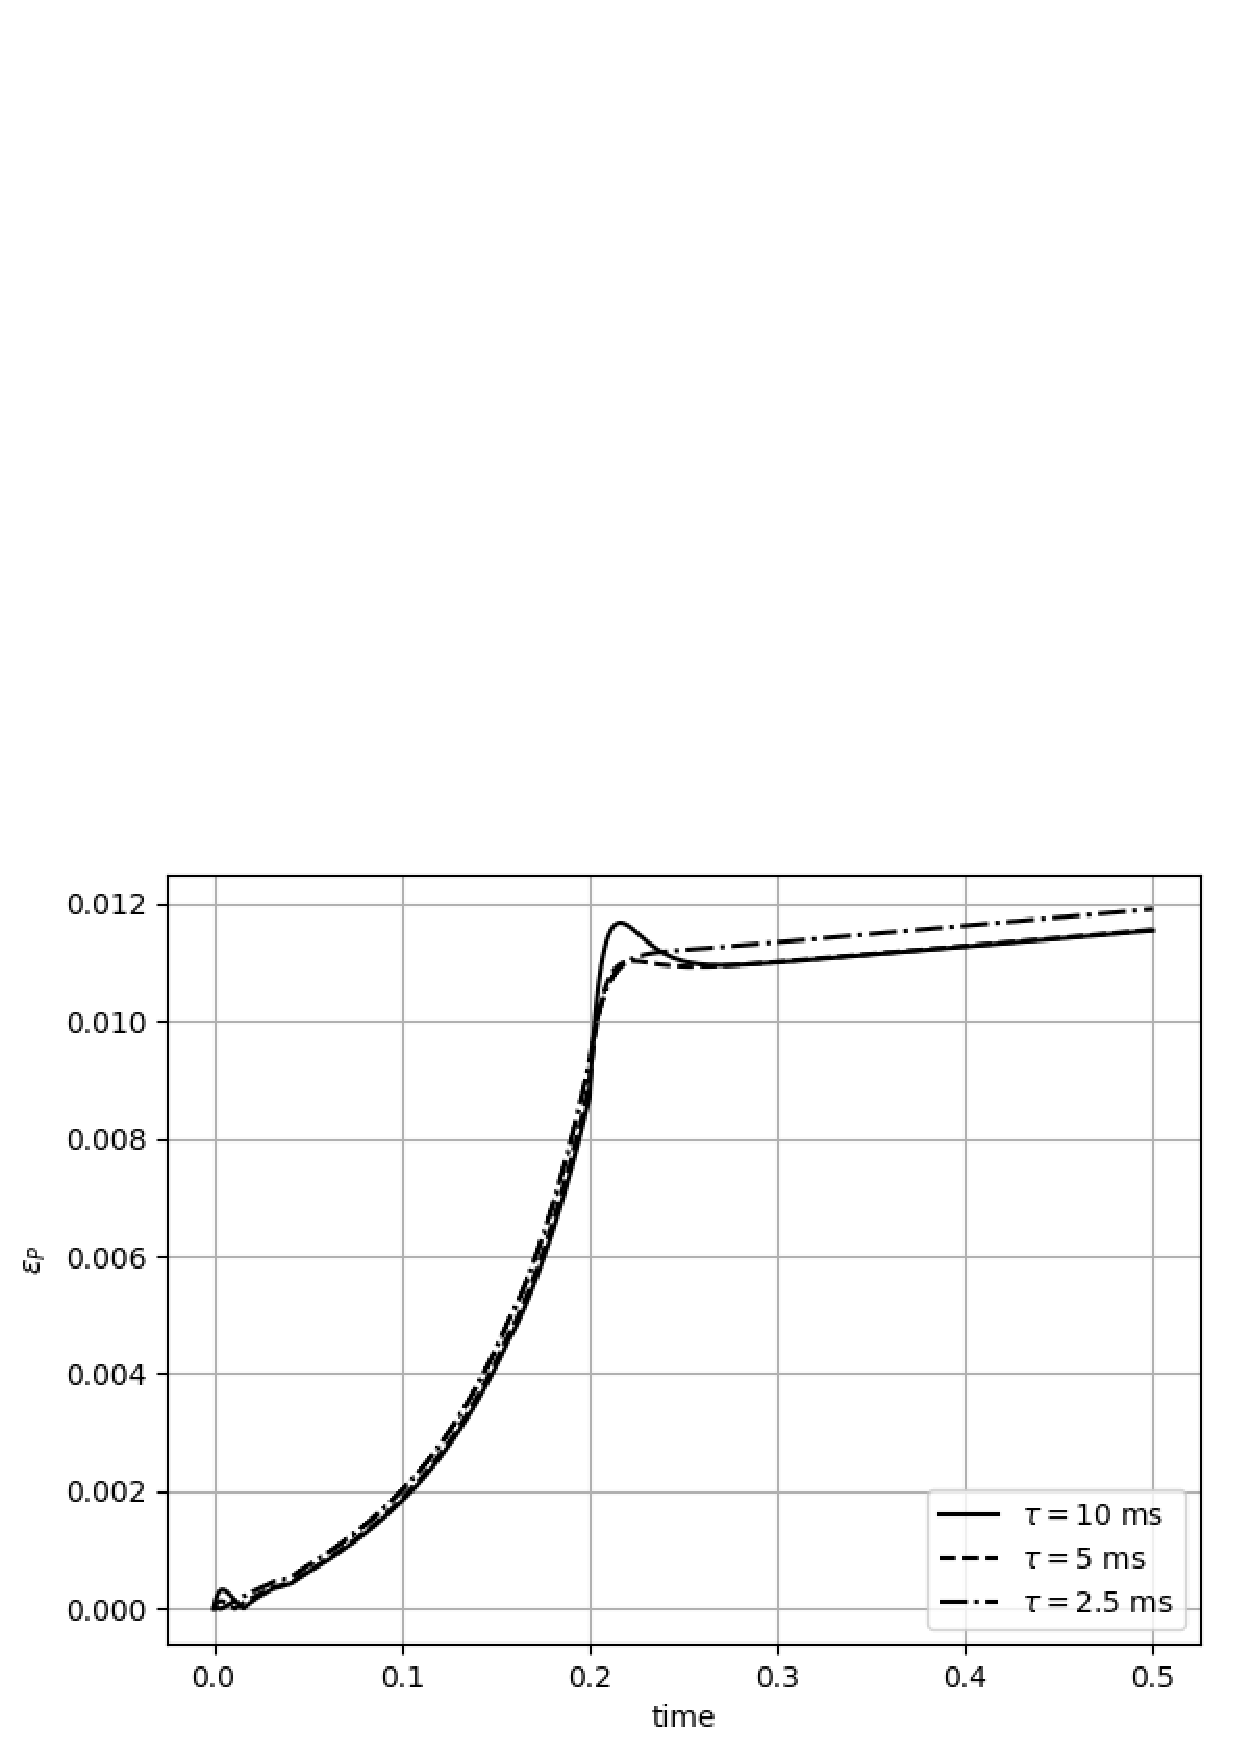
\includegraphics[width=0.5\linewidth]{dif_tau_r.png}\\
	\caption{\label{image:canonsummary}Результаты расчета TWIGL-R для различных шагов по времени по диффузионной модели при $\gamma=0.5$.}
	\label{ris:dif_tau_r_0.5}
\end{center}
\end{figure}

\begin{figure}[ht]
\begin{center}
	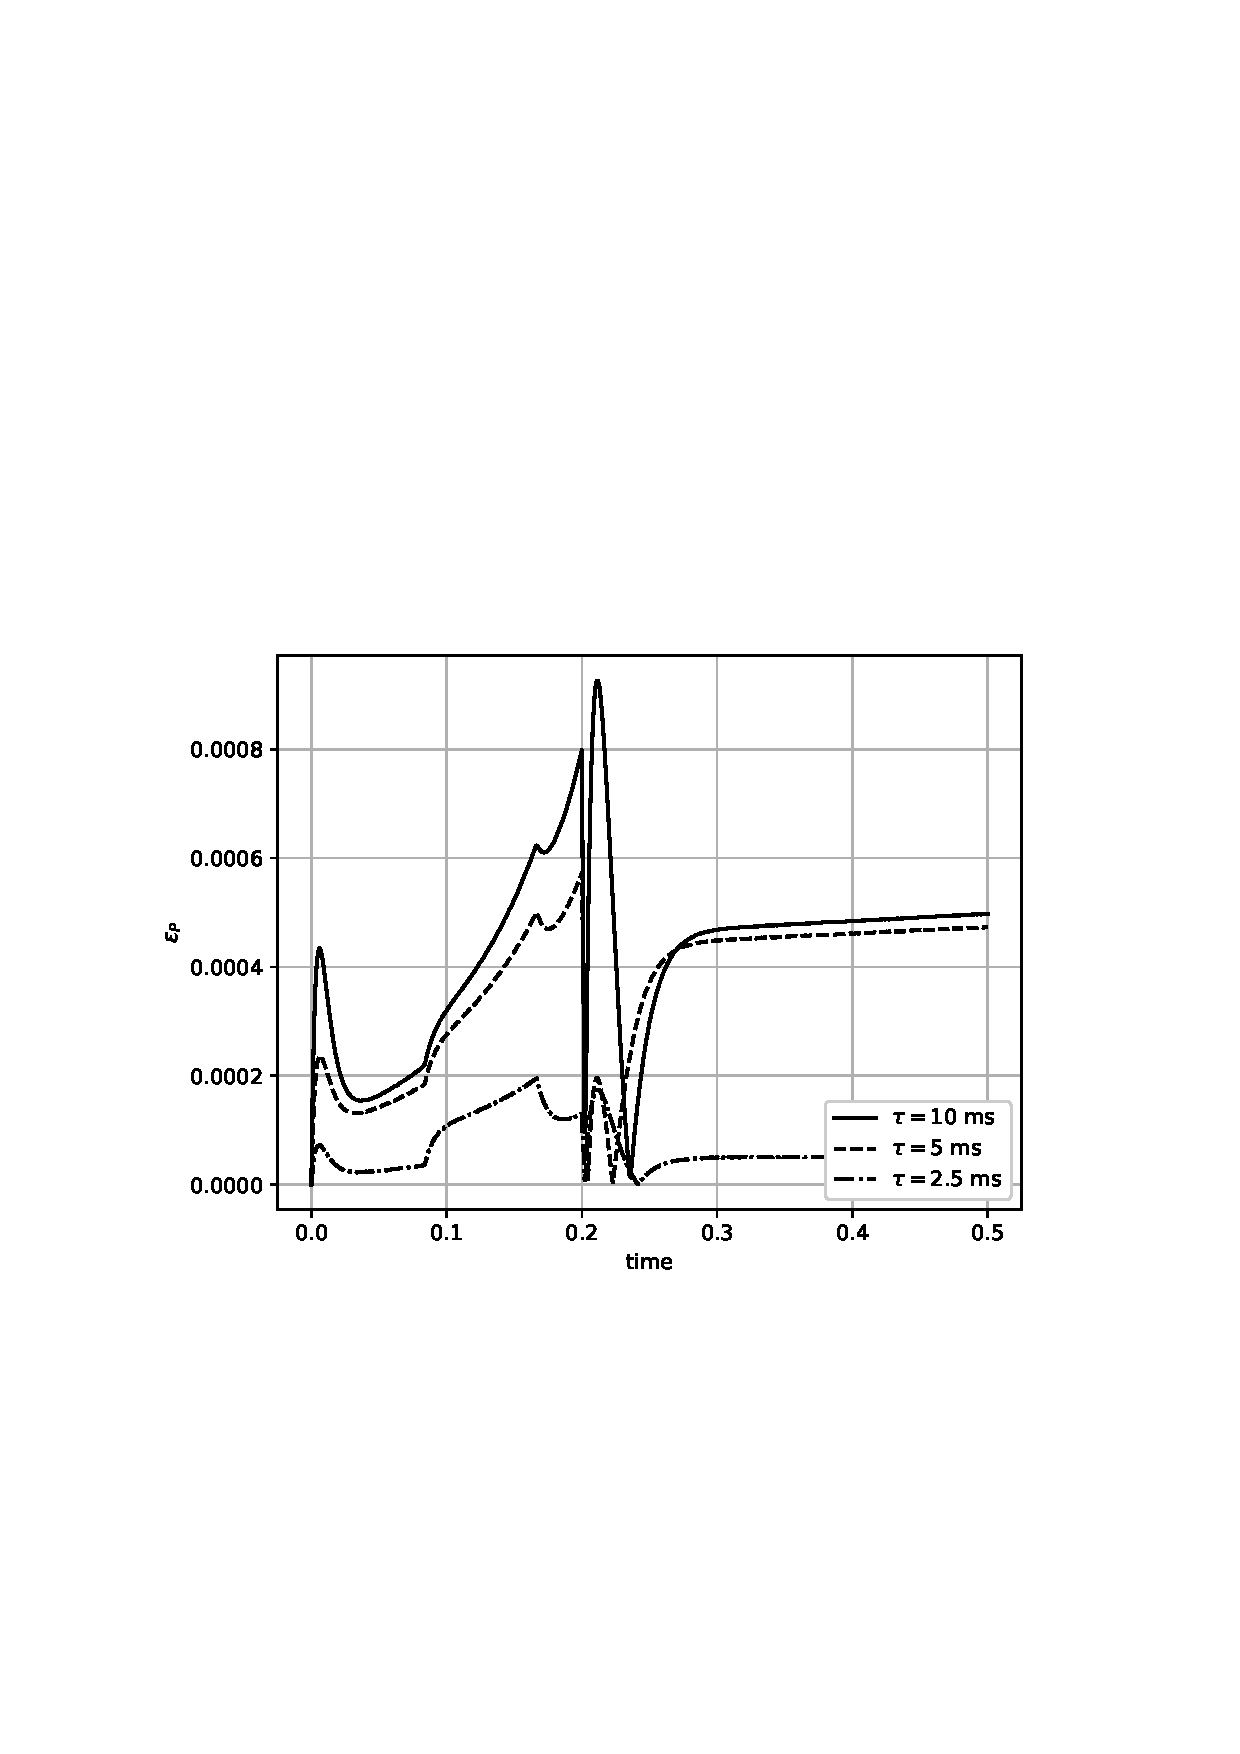
\includegraphics[width=0.5\linewidth]{dif_tau_r_100.png}\\
	\caption{\label{image:canonsummary}Результаты расчета TWIGL-R для различных шагов по времени по диффузионной модели при $\gamma=100$.}
	\label{ris:dif_tau_r_100}
\end{center}
\end{figure}

\begin{figure}[ht]
\begin{center}
	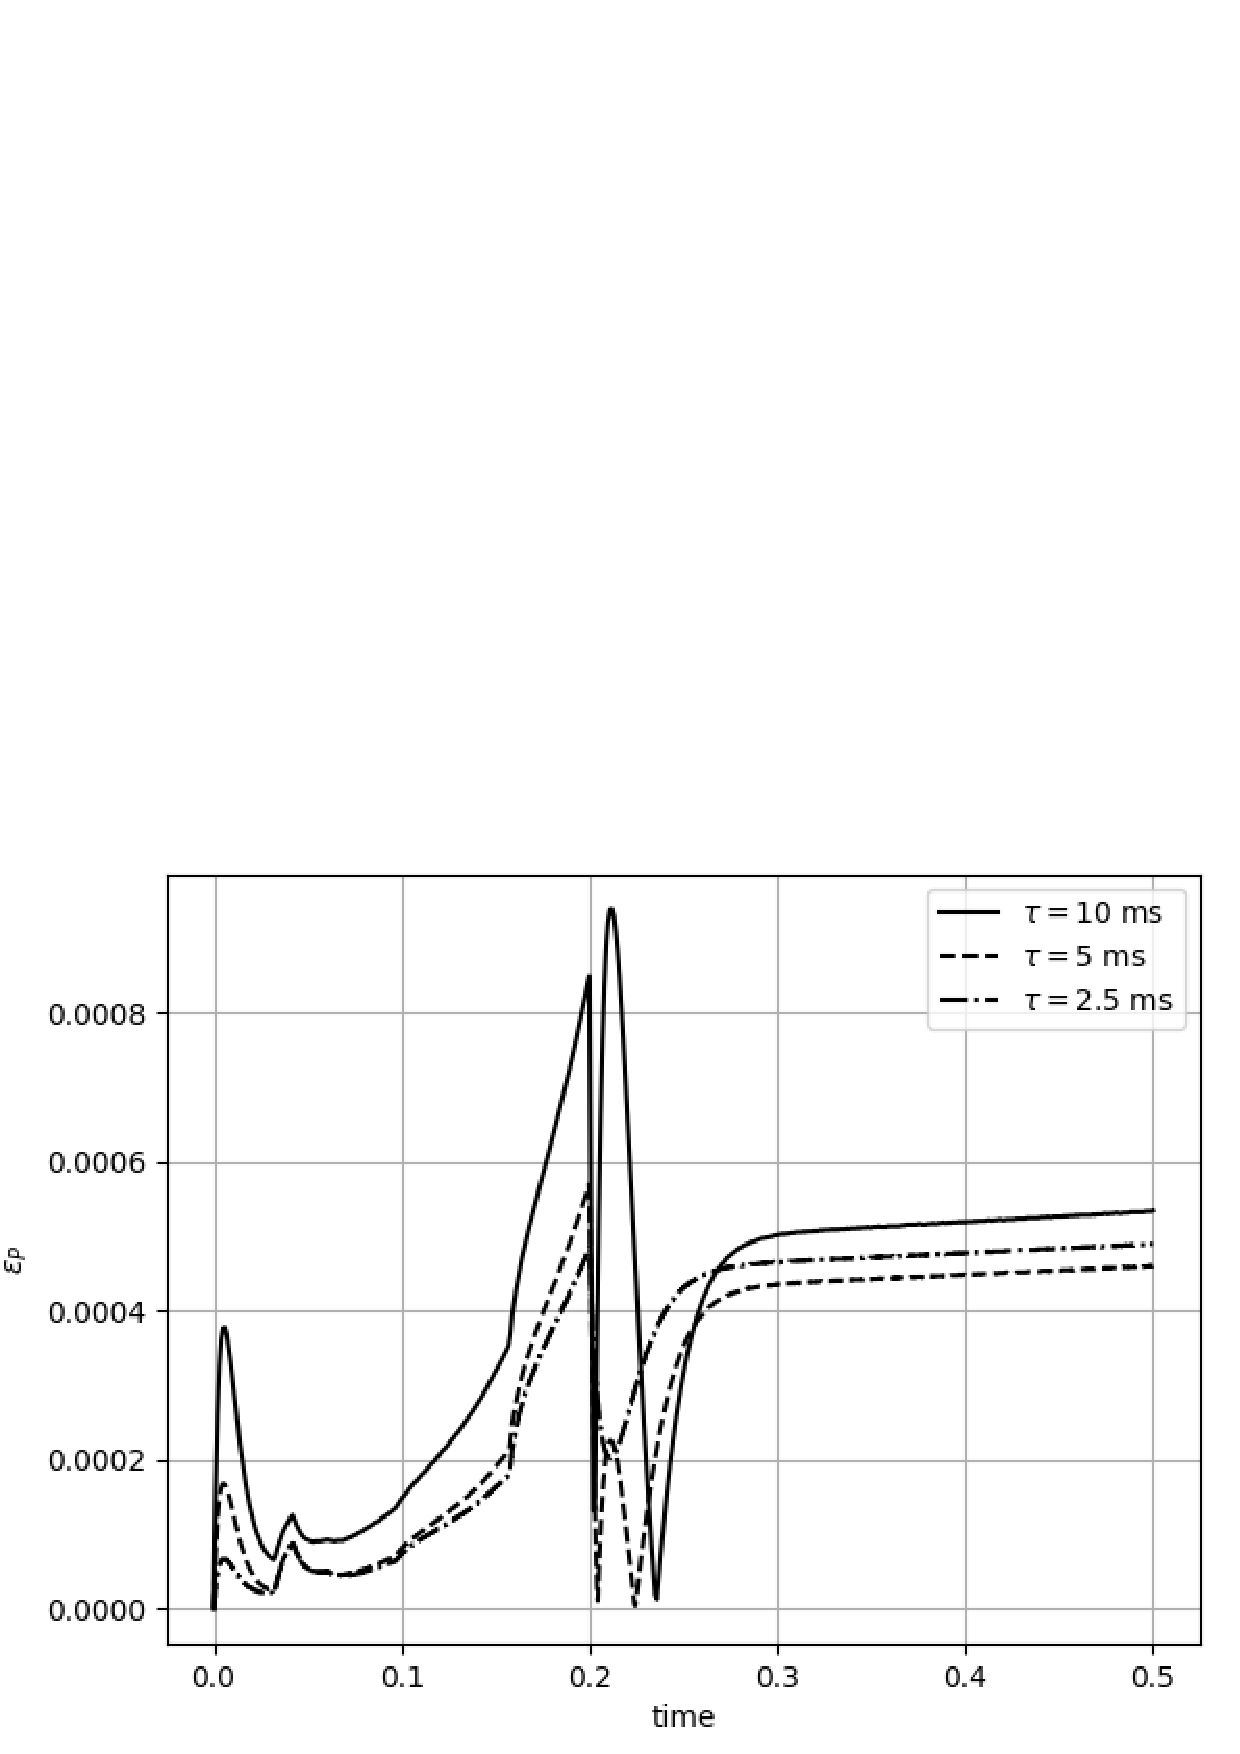
\includegraphics[width=0.5\linewidth]{sp3_tau_r.png}\\
	\caption{\label{image:canonsummary}Результаты расчета TWIGL-R для различных шагов по времени по транспортной sp3 модели.}
	\label{ris:sp3_tau_r}
\end{center}
\end{figure}

\pagebreak
\newpage

\subparagraph{Cценарий №3}
В таблице \ref{table:twigl-c} представлены результаты эталонных решений TWIGL-C при $n=32, p=3, \tau=1$ мс по диффузионной и транспортной моделях.
На рисунке \ref{ris:sp3_ref_c} показано эталонное решение TWIGL-C по транспортной модели, а на рисунке \ref{ris:odds_c} показаны различия диффузионных эталонных решений относительно транспортного эталонного решения. 
Далее, на рисунках \ref{ris:dif_tau_c_0.5}, \ref{ris:dif_tau_c_100}, \ref{ris:sp3_tau_c} показаны отличия при различных шагах по времени относительно эталонных решений.


\begin{table}[htp]
\caption{Различие результатов диффузионного и транспортного расчетов для TWIGL-C.}
\label{table:twigl-c}
\begin{center}
\begin{tabular}{r r r r}
\hline
$t$ & Dif ($\gamma=0.5$) & Dif ($\gamma=100$) & SP$_3$\\
\hline
0.0 & 1.0000 & 1.0000 & 1.0000\\
0.1 & 1.3422  & 1.3393 & 1.3402\\
0.2 & 2.1686  & 2.1580 & 2.1757\\
0.3 & 0.7103  & 0.7119 & 0.7109\\
0.4 & 0.6452 & 0.6470 & 0.6455\\
0.5 & 1.0024  & 1.0024 & 1.0051\\
\hline
\end{tabular}
\end{center}
\end{table}

\begin{figure}[ht]
\begin{center}
	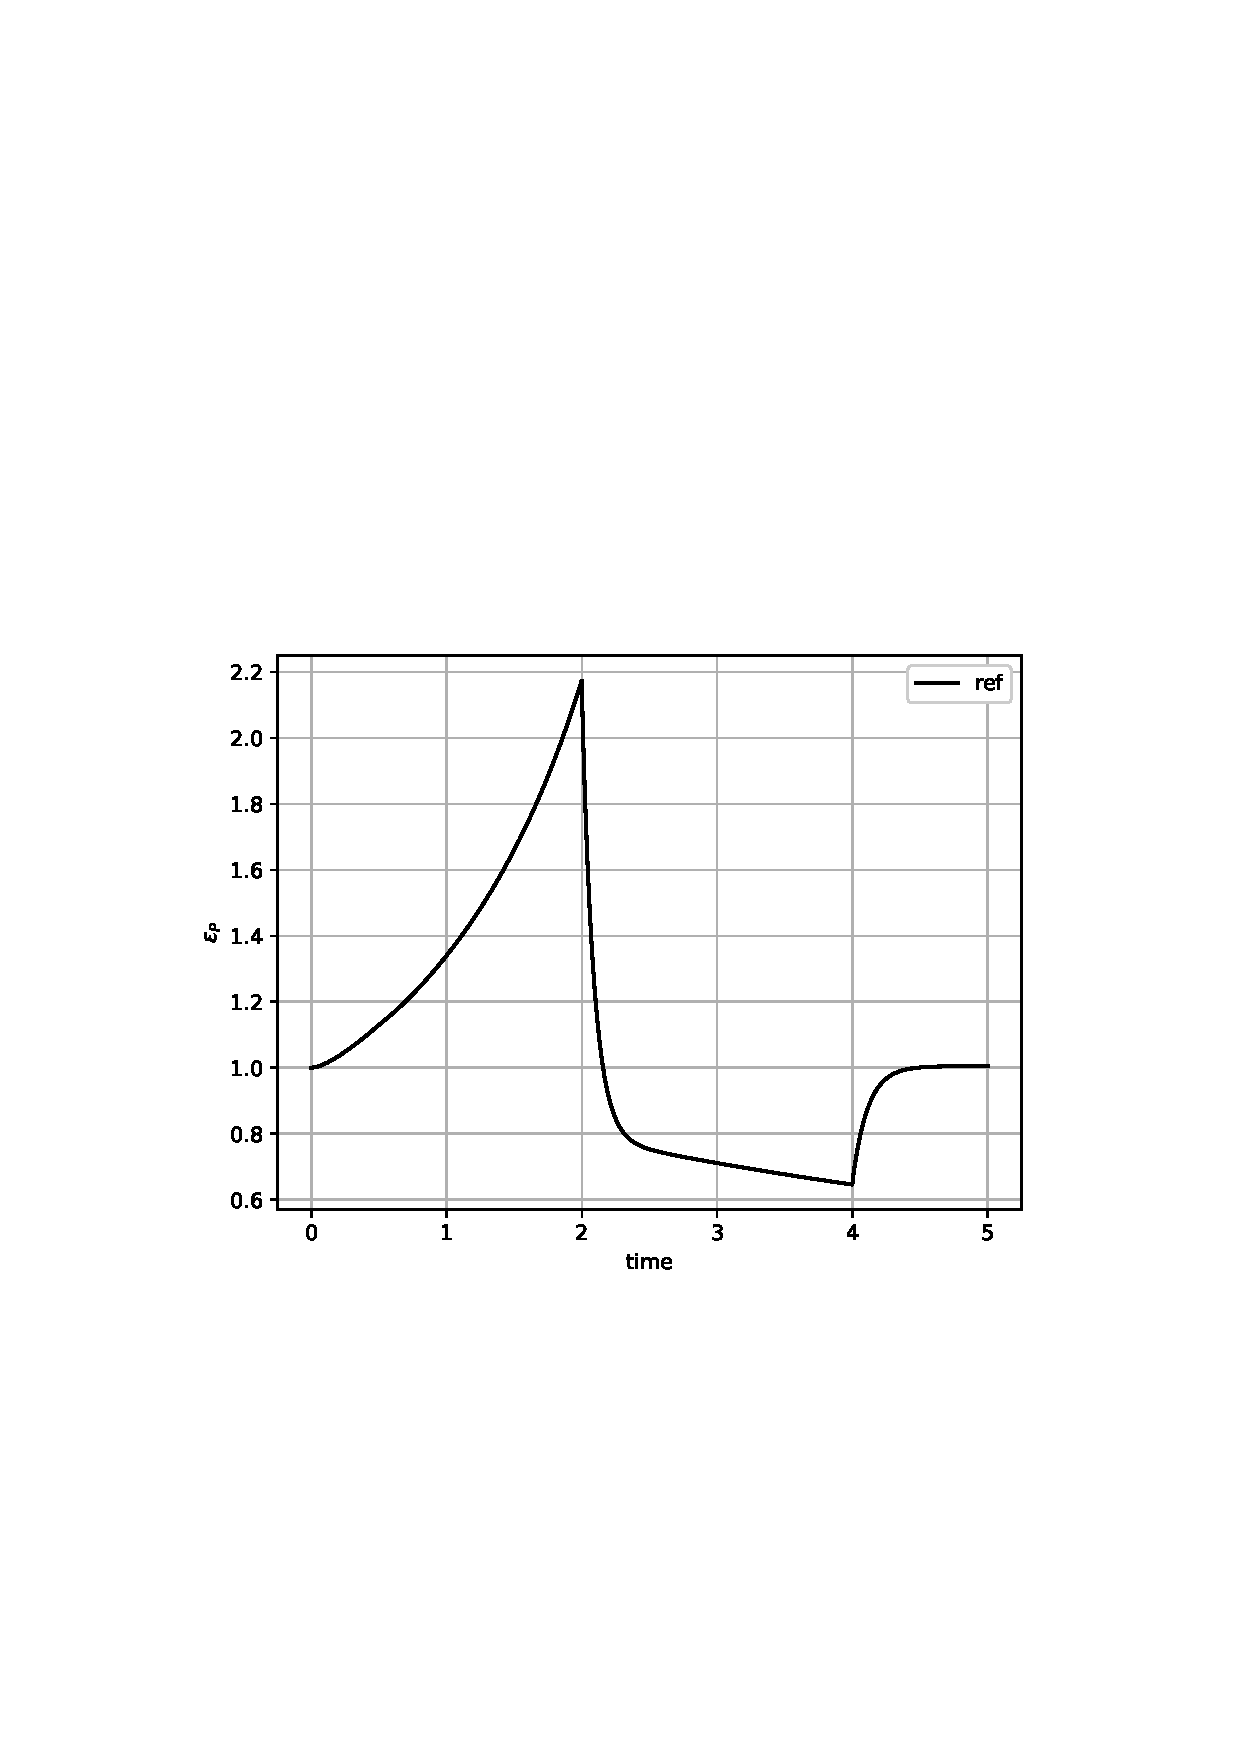
\includegraphics[width=0.5\linewidth]{sp3_ref_c.png}\\
	\caption{\label{image:canonsummary} Эталонное решение TWIGL-C по транспортной SP$_3$ модели.}
	\label{ris:sp3_ref_c}
\end{center}
\end{figure}

\begin{figure}[ht]
\begin{center}
	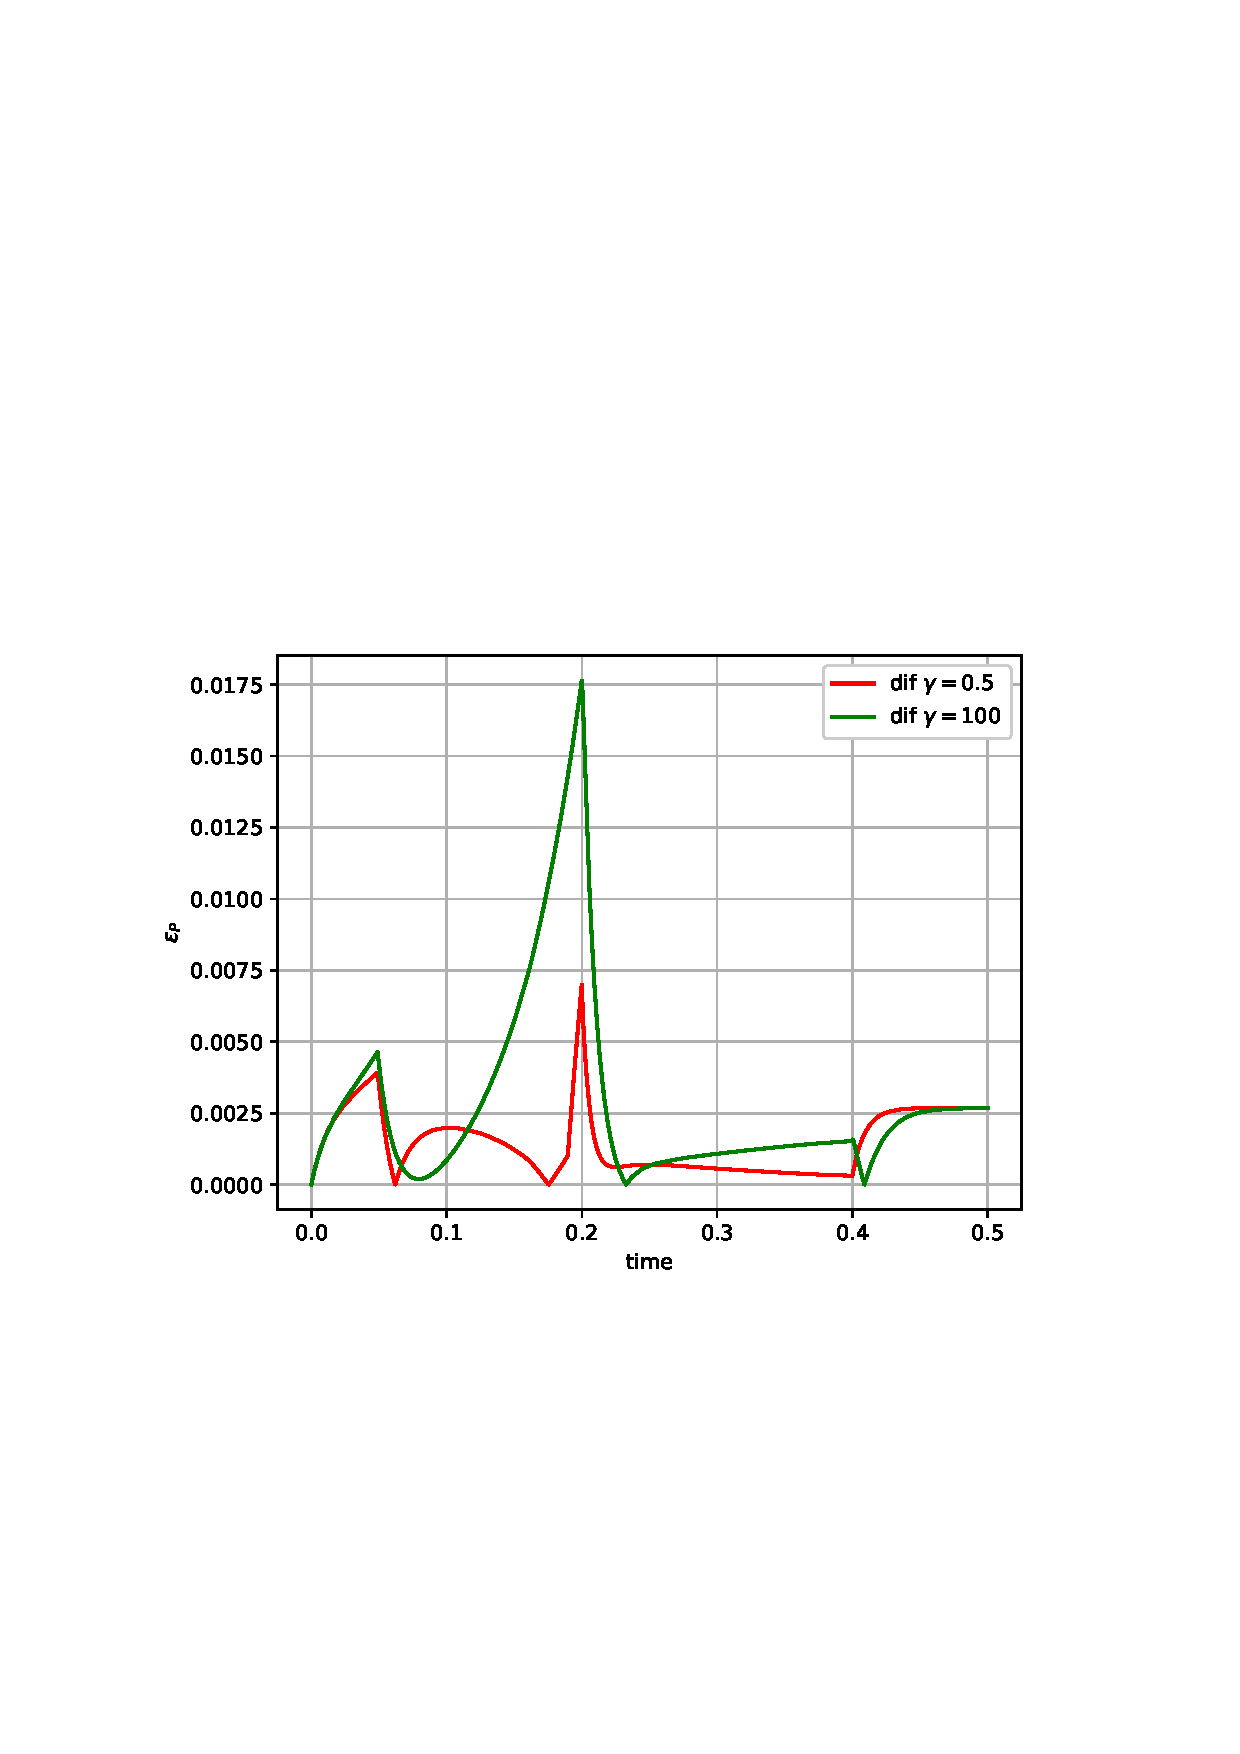
\includegraphics[width=0.5\linewidth]{odds_c.png}\\
	\caption{\label{image:canonsummary} Различия решения TWIGL-C по диффузионной модели от транспортной модели.}
	\label{ris:odds_c}
\end{center}
\end{figure}

\begin{figure}[ht]
\begin{center}
	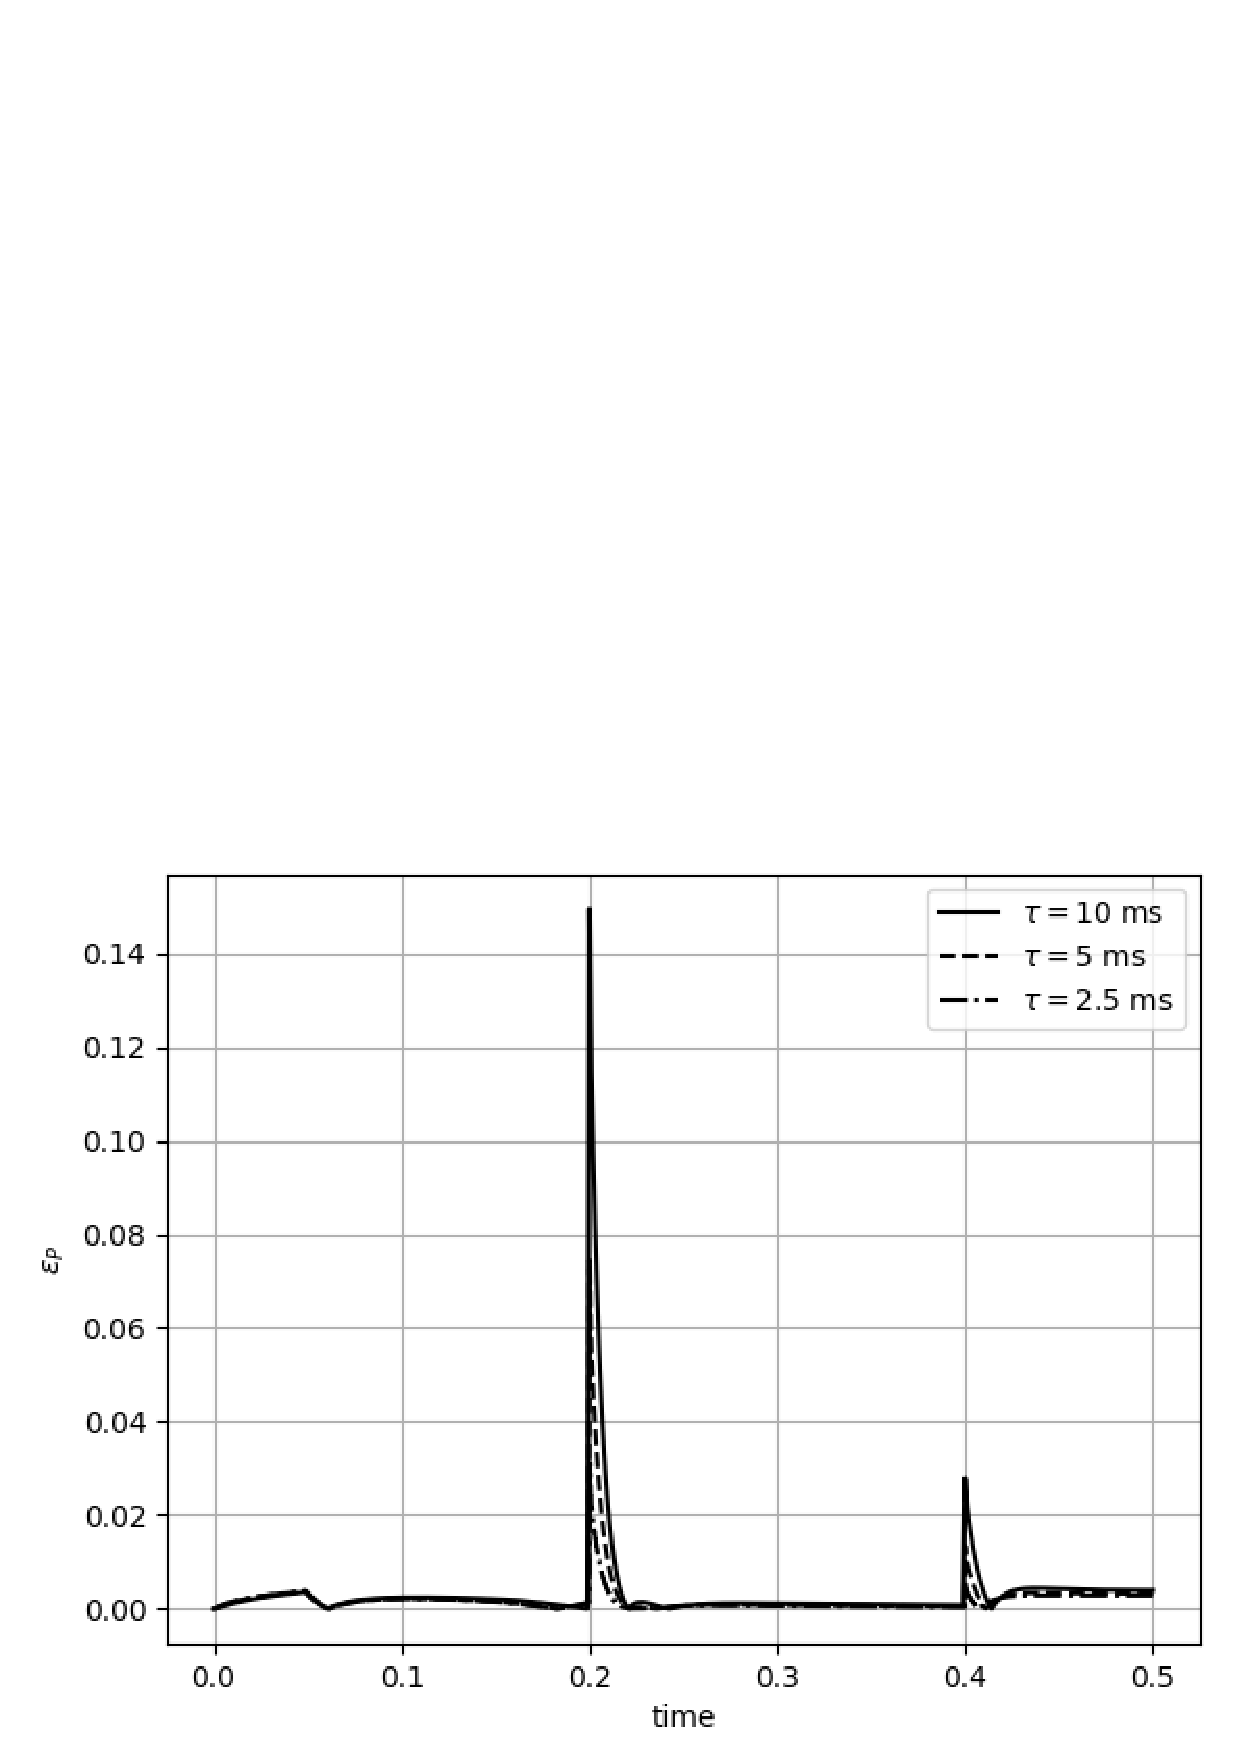
\includegraphics[width=0.5\linewidth]{dif_tau_c.png}\\
	\caption{\label{image:canonsummary}Результаты расчета TWIGL-C для различных шагов по времени по диффузионной модели при $\gamma=0.5$.}
	\label{ris:dif_tau_c_0.5}
\end{center}
\end{figure}

\begin{figure}[ht]
\begin{center}
	\includegraphics[width=0.5\linewidth]{dif_tau_c_100.png}\\
	\caption{\label{image:canonsummary}Результаты расчета TWIGL-C для различных шагов по времени по диффузионной модели при $\gamma=100$.}
	\label{ris:dif_tau_c_100}
\end{center}
\end{figure}

\begin{figure}[ht]
\begin{center}
	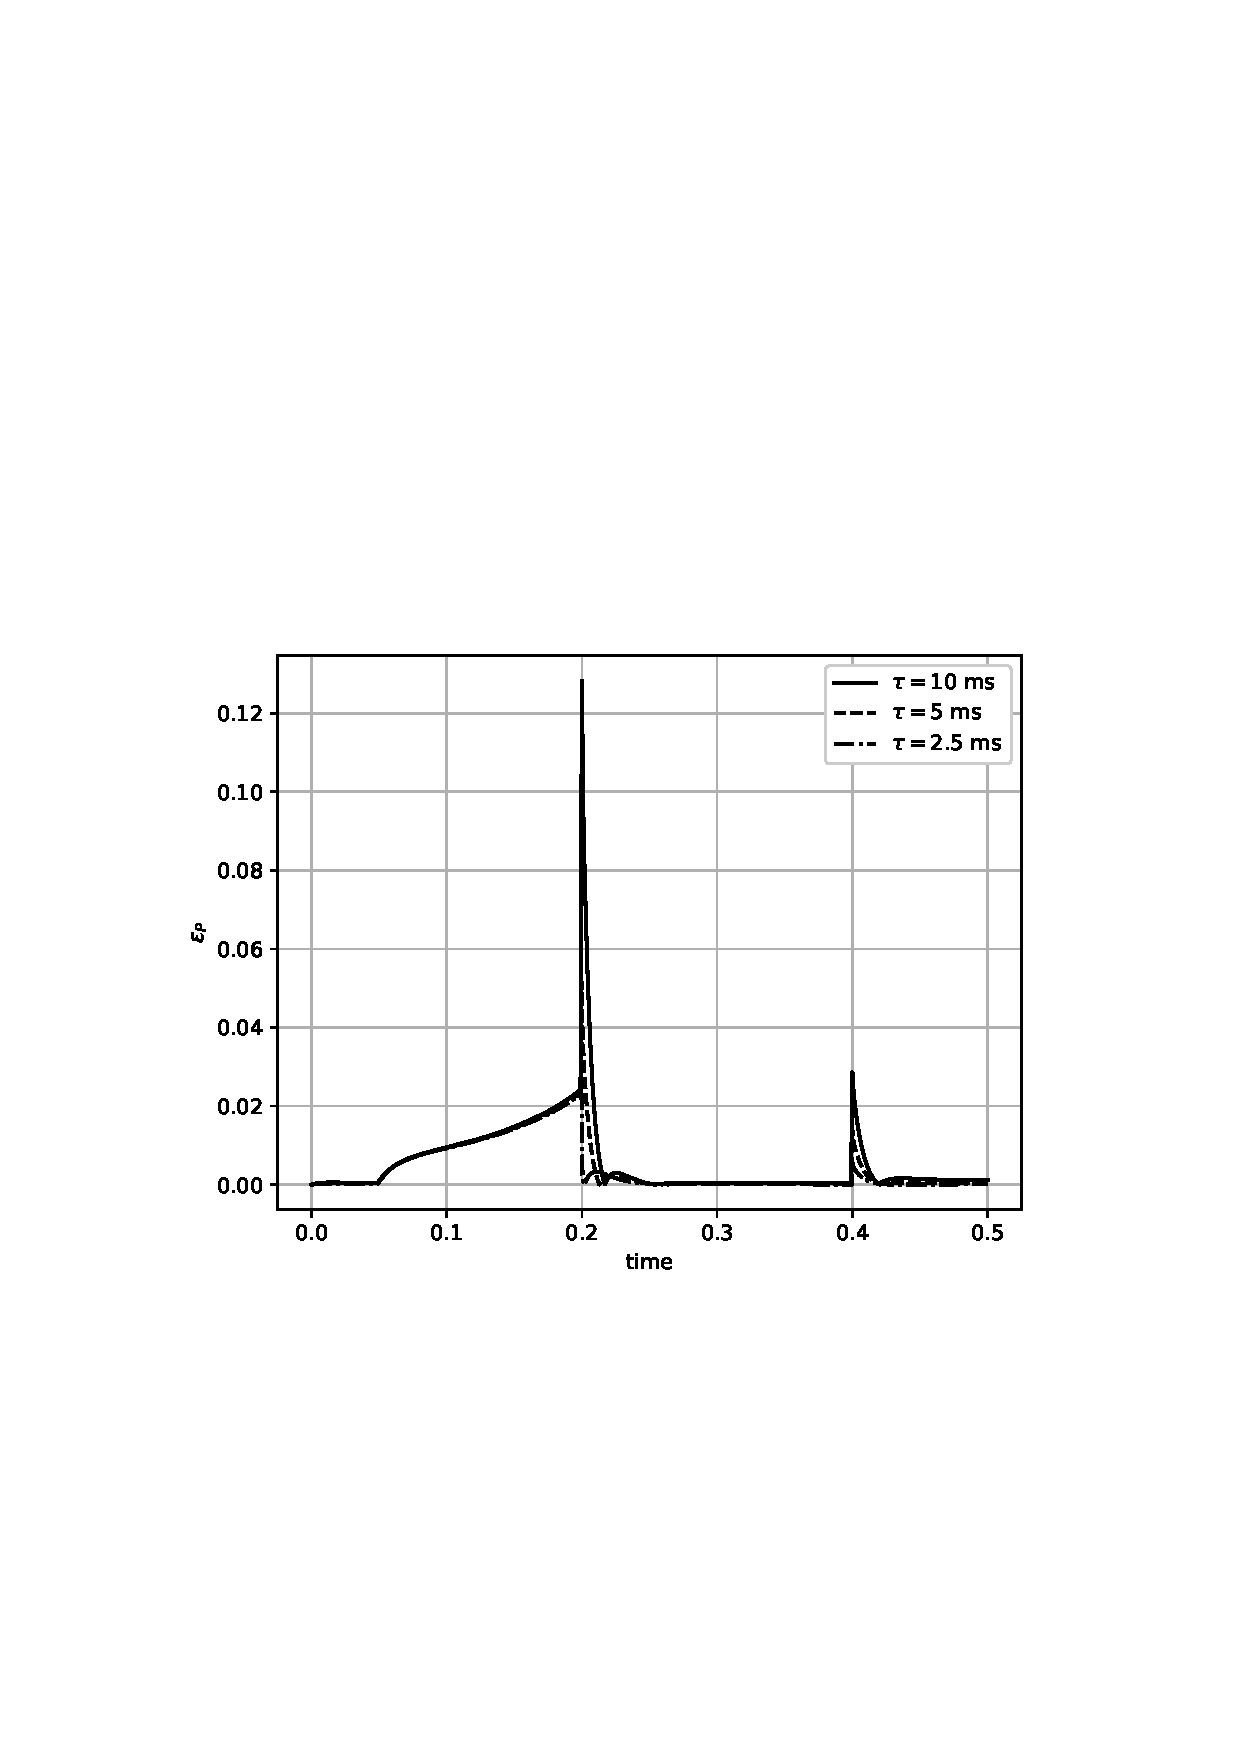
\includegraphics[width=0.5\linewidth]{sp3_tau_c.png}\\
	\caption{\label{image:canonsummary}Результаты расчета TWIGL-C для различных шагов по времени по транспортной sp3 модели.}
	\label{ris:sp3_tau_c}
\end{center}
\end{figure}
%%%%пример оформления списка литературы в соответствии с ГОСТ Р 7.0.5-2008.
	
\paragraph{Заключение}

Simulation of reactor dynamic processes is basically considered on the basis of multigroup diffusion approximation of the neutron transport equation. 
To improve the calculation accuracy for some situations of interest, including pin-by-pin calculations, the $\mathrm{SP_3}$ approximation was adopted in different whole-core diffusion codes as an improved option compared with the diffusion approximation. 
In this regard, it will be very useful to compare the spectral parameters, calculated by both the diffusion and $\mathrm{SP_3}$ options using the finite element method. 

Solution of the $\lambda$- and $\alpha$-spectral problems has been tested for the IAEA-2D and HWR reactor benchmark tests. 
The classical Lagrange finite elements are used for the spatial approximation. 
Accuracy control is performed using condensed grids. 
Spectral problems are solved numerically using well-developed free software SLEPc and using GMSH as a generic mesh generator.

It was found noticeable differences in $\alpha$-eigenvalues problems taking into account delayed neutrons. 
Of particular interest is the problem associated with appearance of complex eigenvalues and eigenfunctions. 
It was found that this tendency occurs for both the diffusion and $\mathrm{SP_3}$ solutions of the HWR reactor test. 
On the contrary, solutions of the IAEA-2D benchmark test showed the absence of complex eigenvalues and eigenfunctions, even in a skew-symmetric variant of the benchmark.

\begin{thebibliography}{99}


\bibitem[Биррелл, Девис, 1984]{Devis} {\it Биррелл~Н., Девис~В.}
    Квантованные поля в искривленном пространстве-времени.~--- М.:
    Мир, 1984.~--- 356~с.\\
%\bibitem[Birrell, Devis, 1984]{devisENG}
{\footnotesize {\em Birrell N. D., Davies P. C. W.} Quantum fields in curved space.~--- Cambridge university press, 1984.~--- No.~7.
(Russ. ed.: {\it Birrell~N., Devis~V.}
    Kvantovannye polya v iskrivlennom prostranstve vremeni.~--- Moskva:
    Mir, 1984~--- 356~s.) \par}

\bibitem[Браун, 1983]{Braun} {\it Браун~П.\,А., Киселев~А.\,А.}
    Введение в теорию молекулярных спектров.~--- Л.: Изд-во Ленингр.
    ун-та, 1938.~--- 232~с.
\\
%\bibitem[Braun, 1983]{BraunENG}
{\footnotesize{\it Braun~P.\,A., Kiselev~A.\,A.}
    Vvedenie v teoriyu molekulyarnyh spektrov [Introduction to the Theory of Molecular Spectra].~--- Leningrad: Izd-vo Leningr.
    un-ta, 1938.~--- 232~s. (in Russian).\par}

\bibitem[Бреев~А.\,И., 2007]{Br07} {\it Бреев~А.\,И., Широков~И.\,В.,
    Разумов~Н.} Поляризация вакуума скалярного поля на многообразии,
    конформно-эквивалентном RхG // Известия высших учебных заведений.
    Физика.~--- 2007.~--- \No~10.~--- C.~50--56.
\\
%\bibitem[breev~A.\,I.,2007]{Br07ENG}
{\footnotesize{\it Breev~A.\,I.,
    Shirokov~I.\,V., Razumov N.} Polyarizaciya vakuuma skalyarnogo
    polya na mnogoobrazii konformno-ehkvivalentnom rhg [Polarization
    of a scalar field vacuum on a manifold conformally equivalent to
    the manifold R$\otimes$ G] // Izvestiya
    vysshih uchebnyh zavedenij. Fizika.~--- 2007.~--- No.~10.~--- S.~50--56 (in Russian).\par}

\bibitem[Гончаровский, 2009]{Gon09} {\it Гончаровский~М.\,М.,
    Широков~И.\,В.} Интегрируемый класс дифференциальных уравнений с
    нелокальной нелинейностью на группах Ли~// Теоретическая и
    математическая физика.~--- Т.~161, \No~3.~--- C. 332--345.
\\
%\bibitem[Goncharovskij,2009]{Gon09ENG}
{\footnotesize{\it Goncharovskij~M.\,M., Shirokov~I.\,V.} Integriruemyj klass differencialnyh uravnenij s
    nelokalnoj nelinejnostyu nagruppah Li [An integrable class of
    differential equations with nonlocal nonlinearity on Lie groups]~// Teoreticheskaya i
    Matematicheskaya Fizika.~--- Vol.~161, No.~3.~--- S.~332--345 (in Russian).\par}



\bibitem[Гриб, Мамаев, 1988]{Grib} {\it Гриб~A.\,A., Мамаев~C.\,Г.,
    Мостепаненко~В.\,М.} Вакуумные квантовые эффекты в сильных
    полях.~--- М.: Атомиздат, 1988.~--- 288~с.
\\
%\bibitem[Grib, Mamaev, 1988]{GribENG}
{\footnotesize{\it Grib~A.\,A.,
    Mamaev~C.\,G., Mostepanenko~V.\,M.} Vakuumnye kvantovye ehffekty
    v silnyh polyah [Vacuum quantum effects in strong fields].~--- Moskva: Atomizdat, 1988.~--- 288~s. (in Russian).\par}

\bibitem[Кириллов, 1978]{kirr} {\it Кириллов~А.\,А.} Элементы теории
    представлений.~--- М.: Наука, 1978.~--- 344~с.
\\
%\bibitem[Kirillov, 1978]{kirrENG}
{\footnotesize{\it Kirillov~A.\,A.} Ehlementy
    teorii predstavlenij [Elements of the Theory of Representations].~--- Moskva: Nauka, 1978.~--- 344~s. (in Russian).\par}

\bibitem[Шаповалов, 1995]{Shap95} {\it Шаповалов~А.\,В.,
    Широков~И.\,В.} Некоммутативное интегрирование линейных
    дифференциальных уравнений  // Теоретическая и математическая
    физика.~--- 1995.~--- Т.~104, \No~2.~--- С.~195--213.
\\
%\bibitem[Shapovalov, 9915]{Shap95ENG}
{\footnotesize{\it Shapovalov~A.\,V.,
    Shirolov~I.\,V.} Nekommutativnoe integrirovanie linejnyh
    differencialnyh uravnenij [Noncommutative integration of linear
    differential equations]~// Teoreticheskaya i matematicheskaya
    fizika.~--- 1995.~--- Vol.~104, No.~2.~--- S.~195--213 (in Russian).\par}


\bibitem[Breev, 2014]{Br14} {\it Breev~A.\,I. Shapovalov~A.\,V.}
    Yang-Mills gauge felds conserving the symmetry algebra of the
    Dirac equation in a homogeneous space~// Journal of Physics:
    Conference Series.~--- 2014.~--- Vol.~563.~--- P.~012004.

\bibitem[Hu, 1973]{Hu1} {\it Hu~B.\,L.} Scalar waves in the Mixmaster
    Universe. I. The Helmholtz equation in a fixed background //
    Phys. Rev.~D.~--- 1973.~--- Vol.~{8}, No.~4.~--- P.~1048--1060.

\bibitem[Hu, 1974]{Hu2} {\it Hu~B.\,L.} Scalar waves in the Mixmaster
    Universe. II. Particle creation~// Phys. Rev.~D.~--- 1974.~--- Vol.~9,
No.~9.~--- P.~3263--3281.

\bibitem[Pritomanov, 1985]{Prit} {\it Pritomanov~S.\,A.} Quantum
    effects in Mixmaster Universe // Phys. Lett.~A.~--- 1985.~--- Vol.~107,
No.~1.~--- P.~33--35.

\bibitem[Ryan, 1975]{Ryan} {\it Ryan~M.\,P., Shepley~L.\,C.}
    Homogeneous relativistic cosmologies.~--- Princeton: Princeton
    series in Physics, 1975.~--- 336~p.


\end{thebibliography}


\end{document}
